% ==============================================================================
\section{Generator Model Selection}
% ==============================================================================

Before establishing baseline performance, we compare three frontier LLMs for CLD edge generation: GPT-4.1 (OpenAI), Sonar-Pro (Perplexity), and Claude Sonnet 4 (Anthropic). All models were evaluated on the same three validation CLDs using identical prompts (Nitai\_C, T=0.7).

\begin{table}[H]
\centering
\caption{Generator Model Comparison: Edge Recovery Performance}
\label{tab:generator_model_comparison}
\begin{threeparttable}
\begin{tabular}{llccccccc}
\toprule
\textbf{Model} & \textbf{CLD} & \textbf{Edges} & \textbf{TP} & \textbf{FP} & \textbf{FN} & \textbf{Precision} & \textbf{Recall} & \textbf{F1} \\
\midrule
GPT-4.1 & Social Norms & 90 & 6 & 9 & 5 & 0.400 & 0.545 & 0.462 \\
GPT-4.1 & Depressive & 182 & 26 & 35 & 8 & 0.426 & 0.765 & \textbf{0.547} \\
GPT-4.1 & Emergency Dept & 1056 & 6 & 120 & 27 & 0.048 & 0.182 & 0.075 \\
\midrule
Sonar-Pro & Social Norms & 89 & 7 & 11 & 4 & 0.389 & 0.636 & \textbf{0.483} \\
Sonar-Pro & Depressive & 178 & 24 & 59 & 10 & 0.289 & 0.706 & 0.410 \\
Sonar-Pro & Emergency Dept & 1051 & 24 & 421 & 9 & 0.054 & 0.727 & 0.100 \\
\midrule
Claude-Sonnet-4 & Social Norms & 90 & 10 & 24 & 1 & 0.294 & 0.909 & 0.444 \\
Claude-Sonnet-4 & Depressive & 182 & 32 & 109 & 2 & 0.227 & 0.941 & 0.366 \\
Claude-Sonnet-4 & Emergency Dept & 1056 & 31 & 655 & 2 & 0.045 & 0.939 & 0.086 \\
\midrule
\multicolumn{9}{l}{\textit{Aggregate (all CLDs combined):}} \\
\textbf{GPT-4.1} & Total & 1328 & 38 & 164 & 40 & \textbf{0.188} & 0.487 & \textbf{0.271} \\
Sonar-Pro & Total & 1318 & 55 & 491 & 23 & 0.101 & 0.705 & 0.176 \\
Claude-Sonnet-4 & Total & 1328 & 73 & 788 & 5 & 0.085 & \textbf{0.936} & 0.155 \\
\bottomrule
\end{tabular}
\begin{tablenotes}
\small
\item \textit{Note.} All models used identical prompts (Nitai\_C variant) and temperature (T=0.7). Single run per model due to API cost constraints.
\item \textbf{Key finding:} GPT-4.1 achieves the best aggregate F1 (0.271) through balanced precision-recall.
\item Claude-Sonnet-4 shows highest recall (0.936) but lowest precision (0.085), generating many false positives.
\item Based on these results, \textbf{GPT-4.1 was selected} as the generator model for all subsequent experiments. Additionally, GPT-4.1 is the only model that provides token-level log probabilities (logits), enabling confidence-based edge filtering.
\end{tablenotes}
\end{threeparttable}
\end{table}

% ==============================================================================
\section{Generator Performance Baseline}
% ==============================================================================

Having selected GPT-4.1 based on the model comparison above, we now establish its baseline performance. These foundational results demonstrate that the CLD generator captures genuine causal structure and that the chosen hyperparameters (T=0.7) are empirically justified.

\subsection{Random Baseline Comparison}

To confirm the generator produces meaningful causal structure rather than random edge configurations, we compare LLM-generated edges against a Monte Carlo random baseline.

\begin{table}[H]
\centering
\caption{Random Baseline Comparison for Generator Edge Recovery}
\label{tab:random_baseline}
\begin{tabular}{lcccccc}
\toprule
\textbf{CLD} & $|V|$ & $|E|$ & \textbf{Density} & \textbf{Random F1 [95\% CI]} & \textbf{LLM F1 [95\% CI]} & \textbf{Improv.} \\
\midrule
Depressive Symptoms & 14 & 34 & 0.187 & 0.186 [0.18, 0.19] & 0.530 [0.48, 0.58] & 2.8$\times$ \\
Social Norms & 11 & 12 & 0.109 & 0.123 [0.12, 0.13] & 0.451 [0.34, 0.56] & 3.7$\times$ \\
Emergency Department & 36 & 66 & 0.052 & 0.055 [0.05, 0.06] & 0.131 [0.09, 0.17] & 2.4$\times$ \\
\midrule
\textit{Average} & -- & -- & -- & 0.121 & 0.370 [0.35, 0.39]$^\dagger$ & 3.1$\times$ \\
\bottomrule
\end{tabular}
\begin{tablenotes}
\small
\item \textit{Note.} Random F1 via Monte Carlo (1000 iterations); LLM F1 from 3 generation runs per CLD (seeds 10, 20, 30).
\item Density = $|E| / (|V| \times (|V|-1))$. Per-CLD 95\% CI uses t-distribution (n=3).
\item $^\dagger$Average CI via error propagation: $SE_{\text{avg}} = \sqrt{SE_1^2 + SE_2^2 + SE_3^2}/3 = 0.010$, yielding $0.370 \pm 0.024$.
\item The LLM generator significantly outperforms random baseline across all CLDs (2.4--3.7$\times$).
\end{tablenotes}
\end{table}

\begin{figure}[H]
\centering
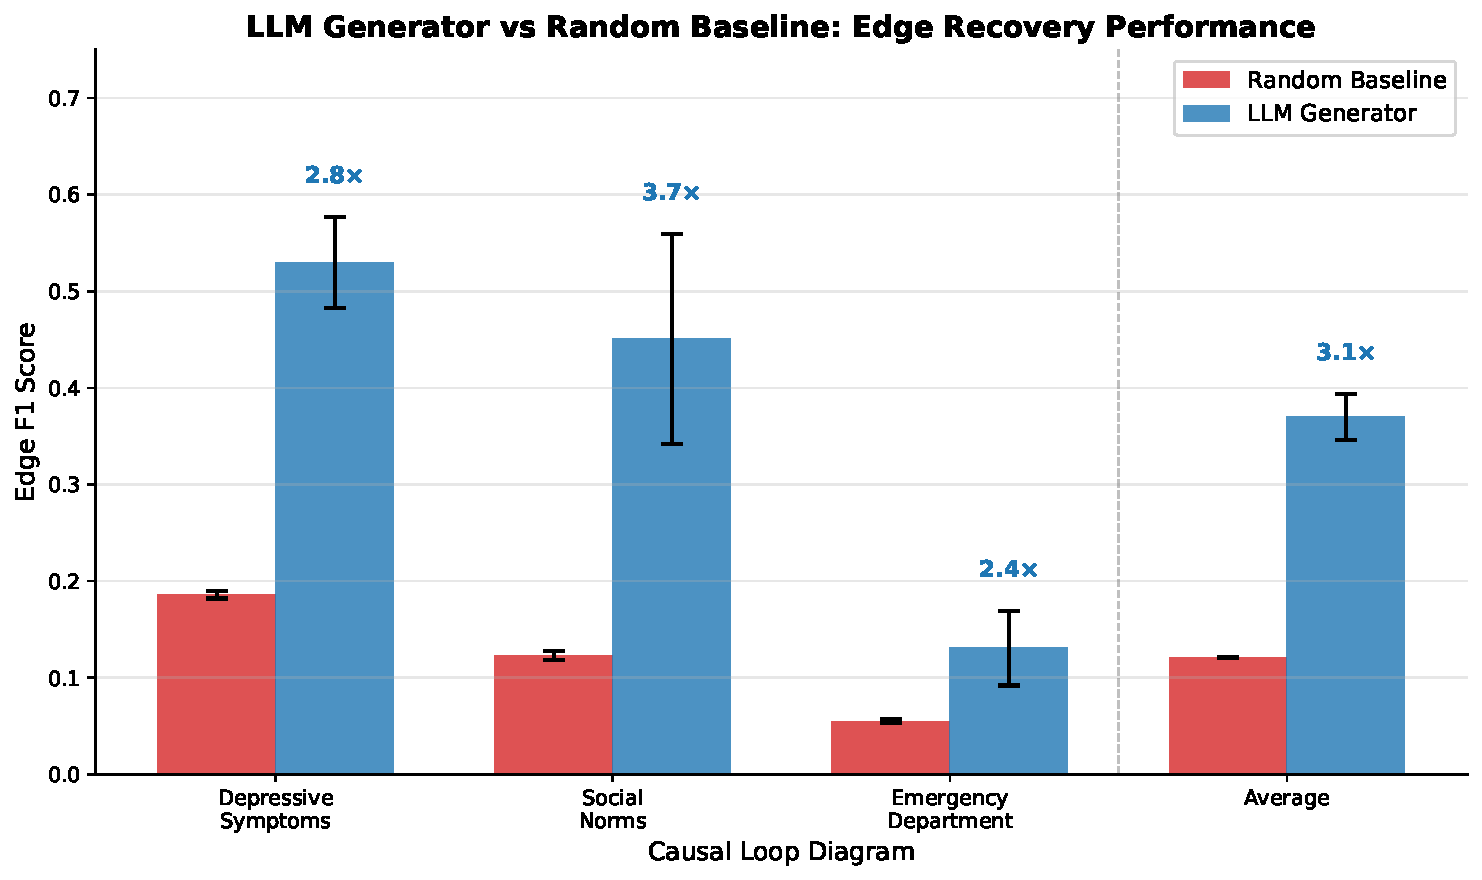
\includegraphics[width=0.9\textwidth]{figures/random_baseline_comparison.pdf}
\caption{LLM generator (GPT-4.1, T=0.7, Nitai\_C prompt) vs.\ random baseline edge F1 across all three validation CLDs. Error bars show 95\% confidence intervals. The LLM consistently outperforms random chance (2.4--3.7$\times$ improvement), confirming the generator captures genuine causal structure. Performance varies by domain complexity: Social Norms shows the largest relative improvement (3.7$\times$) while Emergency Department shows the smallest (2.4$\times$) due to lower absolute F1.}
\label{fig:random_baseline_final}
\end{figure}

\subsection{Temperature Sensitivity Analysis}

To validate the generator temperature choice (T=0.7), we tested whether temperature significantly affects edge recovery performance across all three validation CLDs.

\begin{table}[H]
\centering
\caption{Generator Temperature Sensitivity: Edge F1 Score by CLD}
\label{tab:temperature_sensitivity}
\begin{threeparttable}
\begin{tabular}{lcccc}
\toprule
\textbf{Temperature} & \multicolumn{4}{c}{\textbf{Edge F1 Score (Mean $\pm$ Std)}} \\
\cmidrule(lr){2-5}
 & \textbf{Social Norms} & \textbf{Depressive} & \textbf{Emergency Dept} & \textbf{Overall} \\
\midrule
T=0.0 & $0.342 \pm 0.032$ & $0.455 \pm 0.018$ & $0.110 \pm 0.004$ & $0.302 \pm 0.145$ \\
T=0.3 & $0.305 \pm 0.040$ & $0.445 \pm 0.004$ & $0.109 \pm 0.003$ & $0.286 \pm 0.140$ \\
T=0.5 & $0.333 \pm 0.027$ & $0.479 \pm 0.017$ & $0.123 \pm 0.010$ & $0.312 \pm 0.147$ \\
T=0.7 & $0.329 \pm 0.029$ & $0.445 \pm 0.005$ & $0.109 \pm 0.009$ & $0.294 \pm 0.141$ \\
T=1.0 & $0.347 \pm 0.039$ & $0.444 \pm 0.009$ & $0.109 \pm 0.003$ & $0.300 \pm 0.142$ \\
\bottomrule
\end{tabular}
\begin{tablenotes}
\small
\item \textit{Note.} Edge F1 = $\frac{2 \cdot \text{TP}}{2 \cdot \text{TP} + \text{FP} + \text{FN}}$ comparing generated edges against literature ground truth.
\item \textit{Design.} 5 temperatures $\times$ 3 runs $\times$ 3 CLDs = 45 total experiments. Seeds: 10, 20, 30 per temperature.
\item \textbf{ANOVA:} $F(4,40) = 0.035$, $p = 0.998$, $\eta^2 = 0.004$ (negligible effect).
\item \textit{Assumptions:} Shapiro-Wilk normality and Levene's homogeneity satisfied (all $p > .05$). Result robust: Kruskal-Wallis yields same conclusion.
\item \textbf{Conclusion:} Temperature does not significantly affect Edge F1 ($p > 0.05$), justifying T=0.7 as a reasonable default.
\end{tablenotes}
\end{threeparttable}
\end{table}

% ==============================================================================
\section{Correctness Judge Verification}
% ==============================================================================

Before evaluating the LLM-as-a-Judge approach on CLD edges, we verify that our correctness-based judge implementation has genuine hallucination detection capability using TruthfulQA---a benchmark designed to test whether models can distinguish truthful from false but plausible answers.

\subsection{Classification Performance}

\begin{table}[H]
\centering
\caption{TruthfulQA Judge Verification: Correctness Judge Performance}
\label{tab:truthqa_performance}
\begin{threeparttable}
\begin{tabular}{lcccc}
\toprule
\textbf{Metric} & \textbf{Value} & \textbf{95\% CI} & \textbf{Threshold} & \textbf{Result} \\
\midrule
Accuracy & 87.6\% & [85.9\%, 89.2\%] & $>$80\% & \textcolor{green}{\textbf{PASS}} \\
Precision & 0.890 & [0.866, 0.914] & $>$0.80 & \textcolor{green}{\textbf{PASS}} \\
Recall & 85.9\% & [83.5\%, 88.3\%] & $>$80\% & \textcolor{green}{\textbf{PASS}} \\
F1 Score & 0.874 & [0.853, 0.895] & $>$0.80 & \textcolor{green}{\textbf{PASS}} \\
Specificity & 89.4\% & [87.2\%, 91.5\%] & $>$80\% & \textcolor{green}{\textbf{PASS}} \\
\bottomrule
\end{tabular}
\begin{tablenotes}
\small
\item \textit{Note.} Judge: GPT-4.1, temp=0.0, seed=42, baseline correctness prompt.
\item Dataset: 1,634 samples (817 hallucinated, 817 truthful; 50\% base rate).
\item 95\% CI computed using Wilson score interval.
\item Thresholds based on hypothesis: strong performance = $>$80\% on all metrics.
\end{tablenotes}
\end{threeparttable}
\end{table}

\subsection{Confusion Matrix}

\begin{table}[H]
\centering
\caption{TruthfulQA Confusion Matrix (n=1,634)}
\label{tab:truthqa_confusion}
\begin{threeparttable}
\begin{tabular}{lcc}
\toprule
 & \textbf{Predicted: Hallucinated} & \textbf{Predicted: Truthful} \\
\midrule
\textbf{Actual: Hallucinated} & 702 (TP) & 115 (FN) \\
\textbf{Actual: Truthful} & 87 (FP) & 730 (TN) \\
\bottomrule
\end{tabular}
\begin{tablenotes}
\small
\item \textit{Note.} Classification threshold: judge\_score $<$ 0.5 $\Rightarrow$ Hallucinated.
\item TP = correctly caught hallucinations; FN = missed hallucinations.
\item FP = false alarms (truthful flagged as hallucinated); TN = correctly accepted truthful.
\end{tablenotes}
\end{threeparttable}
\end{table}

\subsection{Key Findings}

\begin{enumerate}[noitemsep]
    \item \textbf{Strong baseline capability:} The correctness judge achieves 87.6\% accuracy and F1=0.874 on TruthfulQA, demonstrating genuine hallucination detection capability.
    \item \textbf{Balanced performance:} Recall (85.9\%) and Specificity (89.4\%) are both high, indicating the judge neither over-flags nor under-flags.
    \item \textbf{High precision:} 89.0\% of flagged hallucinations are actual hallucinations, minimizing false alarms.
\end{enumerate}

\textbf{Interpretation:} This verification establishes that our correctness judge implementation works correctly on a controlled benchmark. The subsequent RQ1a experiments will reveal whether this capability transfers to the more challenging domain of CLD edge validation.

% ==============================================================================
\section{RQ1a: Correctness Judge on Corrupted Edges}
% ==============================================================================

% Path: /home/nitai/code/causalix.ai/final_runs/RQ1a_corruption_detection_correctness_final/enhanced_analysis_20251215_181752/

% NOTE: Full 5-panel aggregate figure available but excluded from final PDF
% File: rq1a_enhanced_visualization.png

\subsection{Performance Metrics Overview}

Detailed view of core performance metrics across all CLDs and prompt variants.

\begin{figure}[H]
\centering

\includegraphics[width=1.0\textwidth]{../../final_runs/RQ1a_corruption_detection_correctness_final/enhanced_analysis_20251215_181752/rq1a_row1_performance_metrics.png}
\caption{Performance metrics overview for correctness-based corruption detection. Shows F1 scores, AUC-ROC with chance baseline, and precision-recall trade-off across all experimental conditions.}
\label{fig:rq1a_correctness_row1}
\end{figure}

\subsection{Detailed Analysis}

In-depth analysis of corruption type detection patterns and score discrimination ability.

\begin{figure}[H]
\centering

\includegraphics[width=1.0\textwidth]{../../final_runs/RQ1a_corruption_detection_correctness_final/enhanced_analysis_20251215_181752/rq1a_row2_detailed_analysis.png}
\caption{Detailed analysis for correctness-based corruption detection. Left: recall by corruption type with color scale from 0.5 to 1.0. Middle: score discrimination showing point-biserial correlation between ground truth and judge scores. Right: classification statistics table showing sample counts (n), percentages, mean judge scores ($\mu$), and 95\% confidence intervals for each prompt type, color-coded by mean score.}
\label{fig:rq1a_correctness_row2}
\end{figure}

\subsection{ROC Curves}

Detailed ROC curves showing discrimination performance for each prompt variant.

\begin{figure}[H]
\centering

\includegraphics[width=1.0\textwidth]{../../final_runs/RQ1a_corruption_detection_correctness_final/enhanced_analysis_20251215_181752/rq1a_roc_curves.png}
\caption{ROC curves for correctness-based corruption detection by prompt. Each subplot shows performance for one prompt variant across all CLDs.}
\label{fig:rq1a_correctness_roc}
\end{figure}

% ==============================================================================
\section{RQ1a: Correctness Judge on Expert Ground Truth}
% ==============================================================================

% Path: /home/nitai/code/causalix.ai/final_runs/RQ1a_ground_truth_correctness/enhanced_analysis_20251215_171302/

% NOTE: Full 6-panel aggregate figure available but excluded from final PDF
% File: rq1a_ground_truth_enhanced_visualization.png

\subsection{Performance Metrics Overview}

Detailed view of core performance metrics across all CLDs and prompt variants.

\begin{figure}[H]
\centering

\includegraphics[width=1.0\textwidth]{../../final_runs/RQ1a_ground_truth_correctness/enhanced_analysis_20251215_171302/rq1a_ground_truth_row1_performance_metrics.png}
\caption{Performance metrics overview for ground truth correctness validation. Shows ROC-AUC with random baseline, F1 scores, and aggregate performance by prompt across all metrics.}
\label{fig:rq1a_gt_correctness_row1}
\end{figure}

\subsection{Detailed Analysis}

In-depth analysis of precision-recall trade-offs, score distributions, and point-biserial correlations.

\begin{figure}[H]
\centering

\includegraphics[width=1.0\textwidth]{../../final_runs/RQ1a_ground_truth_correctness/enhanced_analysis_20251215_171302/rq1a_ground_truth_row2_detailed_analysis.png}
\caption{Detailed analysis for ground truth correctness validation. Left: precision-recall trade-off. Center: score distributions by classification type. Right: point-biserial correlations showing discrimination ability.}
\label{fig:rq1a_gt_correctness_row2}
\end{figure}

\subsection{Score Heatmap}

Detailed score patterns across all experimental conditions.

\begin{figure}[H]
\centering

\includegraphics[width=1.0\textwidth]{../../final_runs/RQ1a_ground_truth_correctness/enhanced_analysis_20251215_171302/rq1a_ground_truth_score_heatmap.png}
\caption{Score heatmap for ground truth correctness validation showing classification scores across CLD × prompt combinations.}
\label{fig:rq1a_gt_correctness_heatmap}
\end{figure}

% ==============================================================================
\section{RQ1a: Citation Judge on Corrupted Edges}
% ==============================================================================

% Path: /home/nitai/code/causalix.ai/final_runs/RQ1a_corruption_detection_citation_gpt5mini/enhanced_analysis_20251219_003752/

% NOTE: Full 5-panel aggregate figure available but excluded from final PDF
% File: rq1a_enhanced_visualization.png

\subsection{Performance Metrics Overview}

Detailed view of core performance metrics across all CLDs and four prompt variants (Baseline, Mechanistic, CoT, Mechanistic-Lit).

\begin{figure}[H]
\centering

\includegraphics[width=1.0\textwidth]{../../final_runs/RQ1a_corruption_detection_citation_gpt5mini/enhanced_analysis_20251219_003752/rq1a_row1_performance_metrics.png}
\caption{Performance metrics overview for citation-based corruption detection. Shows F1 scores, AUC-ROC with chance baseline, and precision-recall trade-off across all experimental conditions (4 prompt variants $\times$ 3 CLDs $\times$ 3 runs = 36 experiments).}
\label{fig:rq1a_citation_row1}
\end{figure}

\subsection{Detailed Analysis}

In-depth analysis of corruption type detection patterns and score discrimination ability.

\begin{figure}[H]
\centering

\includegraphics[width=1.0\textwidth]{../../final_runs/RQ1a_corruption_detection_citation_gpt5mini/enhanced_analysis_20251219_003752/rq1a_row2_detailed_analysis.png}
\caption{Detailed analysis for citation-based corruption detection. Left: recall by corruption type with color scale from 0.5 to 1.0. Middle: score discrimination showing point-biserial correlation between ground truth and judge scores. Right: classification statistics table showing sample counts (n), percentages, mean judge scores ($\mu$), and 95\% confidence intervals for each prompt type, color-coded by mean score.}
\label{fig:rq1a_citation_row2}
\end{figure}

\subsection{ROC Curves}

Detailed ROC curves showing true positive rate vs false positive rate for each prompt variant across all CLDs.

\begin{figure}[H]
\centering

\includegraphics[width=1.0\textwidth]{../../final_runs/RQ1a_corruption_detection_citation_gpt5mini/enhanced_analysis_20251219_003752/rq1a_roc_curves.png}
\caption{ROC curves for citation-based corruption detection by prompt. Each subplot shows performance for one of four prompt variants (Baseline, Mechanistic, CoT, Mechanistic-Lit) across all three CLDs. Curves above the diagonal (chance line) indicate better-than-random discrimination.}
\label{fig:rq1a_citation_roc}
\end{figure}

% ==============================================================================
\section{RQ1a: Citation Judge on Expert Ground Truth}
% ==============================================================================

% Path: /home/nitai/code/causalix.ai/final_runs/RQ1a_ground_truth_citation/enhanced_analysis_20251215_171324/

% NOTE: Full 6-panel aggregate figure available but excluded from final PDF
% File: rq1a_ground_truth_enhanced_visualization.png

\subsection{Performance Metrics Overview}

Detailed view of core performance metrics across all CLDs and prompt variants.

\begin{figure}[H]
\centering

\includegraphics[width=1.0\textwidth]{../../final_runs/RQ1a_ground_truth_citation/enhanced_analysis_20251215_171324/rq1a_ground_truth_row1_performance_metrics.png}
\caption{Performance metrics overview for ground truth citation validation. Shows ROC-AUC with random baseline, F1 scores, and aggregate performance by prompt across all metrics.}
\label{fig:rq1a_gt_citation_row1}
\end{figure}

\subsection{Detailed Analysis}

In-depth analysis of precision-recall trade-offs, score distributions, and point-biserial correlations.

\begin{figure}[H]
\centering

\includegraphics[width=1.0\textwidth]{../../final_runs/RQ1a_ground_truth_citation/enhanced_analysis_20251215_171324/rq1a_ground_truth_row2_detailed_analysis.png}
\caption{Detailed analysis for ground truth citation validation. Left: precision-recall trade-off. Center: score distributions by classification type. Right: point-biserial correlations showing discrimination ability.}
\label{fig:rq1a_gt_citation_row2}
\end{figure}

\subsection{Score Heatmap}

Detailed heatmap showing judge score patterns by classification type across all CLD and prompt combinations.

\begin{figure}[H]
\centering

\includegraphics[width=1.0\textwidth]{../../final_runs/RQ1a_ground_truth_citation/enhanced_analysis_20251215_171324/rq1a_ground_truth_score_heatmap.png}
\caption{Score heatmap for ground truth citation validation. Shows mean judge scores with 95\% confidence intervals for each classification type (TP, TN, FP, FN) across all CLD × prompt combinations.}
\label{fig:rq1a_gt_citation_heatmap}
\end{figure}

% ==============================================================================
\section{RQ1a: External Validation on Ulemans Expert CLD}
% ==============================================================================

To validate the citation-based judge on an independently expert-validated dataset, we evaluated the judge on the Ulemans Alzheimer's disease CLD---a 150-edge causal model constructed through Group Model Building with 17 domain experts. This external validation tests whether the judge performance generalizes beyond our three primary CLDs and assesses the impact of search provider and citation fetcher choices.

\subsection{Search Provider Comparison}

We compared four academic search providers (OpenAlex, Brave, Perplexity, PubMed) combined with two citation fetching methods (Jina AI Reader, ContentScraper) to assess infrastructure impact on judge scores.

\begin{table}[H]
\centering
\caption{Search Provider Comparison on Ulemans Expert CLD (150 edges)}
\label{tab:ulemans_search_providers}
\begin{threeparttable}
\begin{tabular}{lcccccc}
\toprule
\textbf{Provider} & \textbf{Jina AI} & \textbf{ContentScraper} & \textbf{Jina Edges} & \textbf{CS Edges} & \textbf{Jina} & \textbf{CS} \\
 & \textbf{Avg Score} & \textbf{Avg Score} & \textbf{w/ Citations} & \textbf{w/ Citations} & \textbf{Coverage} & \textbf{Coverage} \\
\midrule
OpenAlex & 0.232 & 0.381 & 150/150 & 59/150 & 100.0\% & 39.3\% \\
Brave (no whitelist) & 0.296 & 0.326 & 150/150 & 134/150 & 100.0\% & 89.3\% \\
Brave (whitelist) & 0.290 & 0.329 & 150/150 & 134/150 & 100.0\% & 89.3\% \\
Perplexity & 0.278 & 0.335 & 150/150 & 120/150 & 100.0\% & 80.0\% \\
PubMed & 0.306 & 0.283 & 127/150 & 120/150 & 84.7\% & 80.0\% \\
\bottomrule
\end{tabular}
\begin{tablenotes}
\small
\item \textit{Note.} Jina AI Reader = paywall-bypassing document fetcher; ContentScraper = standard web scraper.
\item Coverage = percentage of edges with successfully fetched citation content.
\item Score Difference = ContentScraper Avg Score $-$ Jina AI Avg Score.
\item \textbf{Key findings:} (1) Jina AI achieves 100\% coverage (vs.\ 39--89\% for ContentScraper) by bypassing paywalls; (2) ContentScraper scores 10--15\% higher when it succeeds, suggesting paywalled content may be less relevant; (3) PubMed achieves highest Jina score (0.306) but lowest coverage (84.7\%); (4) All scores are low ($<$0.4), consistent with RQ1a GT Lit results showing judges struggle with expert-validated CLDs.
\item \textbf{Interpretation:} Low expert CLD scores are infrastructure-invariant---they persist across all provider/fetcher combinations, confirming the fundamental validation gap rather than a retrieval artifact.
\end{tablenotes}
\end{threeparttable}
\end{table}

\subsection{Key Finding}

The Ulemans expert CLD receives uniformly low judge scores (0.23--0.38) across all search provider and fetcher configurations. This external validation confirms that the judge's difficulty with expert-validated CLDs (observed in RQ1a GT Lit experiments) generalizes to independently constructed expert models and is not attributable to search infrastructure choices.

% ==============================================================================
\section{RQ1a: Human-LLM Agreement Validation}
% ==============================================================================

To validate LLM judge reliability, we measured inter-rater agreement between citation-based LLM judges and a domain expert (Mick) across 72 causal edges from 3 independent datasets.

\subsection{Per-Dataset and Combined Agreement}

\begin{table}[H]
\centering
\caption{Human Validation: LLM Judge vs.\ Expert Inter-Rater Agreement}
\label{tab:human_validation}
\begin{threeparttable}
\begin{tabular}{llccccc}
\toprule
\textbf{Dataset} & \textbf{Generator} & \textbf{n} & \textbf{Cohen's $\kappa$} & \textbf{Agreement} & \textbf{Pearson $r$} & \textbf{Interpretation} \\
\midrule
File 1 (Depressive) & GPT-4.1 & 30 & 0.435 & 70.0\% & 0.527** & Moderate \\
File 2 (Depressive) & Claude 4 Sonnet & 30 & 0.792 & 90.0\% & --- & Substantial \\
File 3 (Social norms) & GPT-4.1 & 12 & 0.273 & 50.0\% & --- & Fair \\
\midrule
\textbf{Combined} & \textbf{2 models} & \textbf{72} & \textbf{0.618} & \textbf{80.6\%} & \textbf{0.732***} & \textbf{Substantial} \\
\midrule
Human baseline & N/A (expert) & 13 & $\sim$0.60 & 80.0\% & --- & Substantial \\
\bottomrule
\end{tabular}
\begin{tablenotes}
\small
\item \textit{Note.} Inter-rater reliability between LLM citation judge (GPT-4.1, temp=0.0) and domain expert.
\item Verdicts: Not supported (0), Partially supported (0.5), Fully supported (1).
\item $\kappa$ interpretation (Landis \& Koch, 1977): $<$0.20 slight, 0.21--0.40 fair, 0.41--0.60 moderate, 0.61--0.80 substantial, $>$0.80 almost perfect.
\item Human baseline from prior GMB validation studies on comparable expert tasks.
\item Significance: ** $p<0.01$, *** $p<0.001$. Pearson $r$ unavailable for Files 2--3 due to limited score variance.
\end{tablenotes}
\end{threeparttable}
\end{table}

\subsection{Disagreement Analysis}

\begin{table}[H]
\centering
\caption{Confusion Matrix: LLM Judge vs.\ Human Expert (Combined, n=72)}
\label{tab:human_validation_confusion}
\begin{threeparttable}
\begin{tabular}{lccc}
\toprule
 & \textbf{LLM: Not supported} & \textbf{LLM: Partially} & \textbf{LLM: Fully} \\
\midrule
\textbf{Human: Not supported} & 37 (51.4\%) & 11 (15.3\%) & 0 (0\%) \\
\textbf{Human: Partially} & 0 (0\%) & 21 (29.2\%) & 3 (4.2\%) \\
\textbf{Human: Fully} & 0 (0\%) & 0 (0\%) & 0 (0\%) \\
\bottomrule
\end{tabular}
\begin{tablenotes}
\small
\item \textit{Note.} Rows = human expert verdicts; columns = LLM judge verdicts.
\item \textbf{Key finding:} 14 disagreements (19.4\%), all showing LLM more lenient than human:
\item \quad -- 11 cases: LLM said ``Partially'' when human said ``Not supported''
\item \quad -- 3 cases: LLM said ``Fully'' when human said ``Partially''
\item \textbf{Zero false negatives:} LLM never under-estimated evidence support.
\end{tablenotes}
\end{threeparttable}
\end{table}

\subsection{Key Findings}

\begin{enumerate}[noitemsep]
    \item \textbf{Substantial combined agreement} ($\kappa=0.618$, 80.6\%) across 72 edges demonstrates LLM judges reliably assess citation support
    \item \textbf{Strong correlation} ($r=0.732$, $p<0.001$) between LLM and human scores
    \item \textbf{Meets human baseline:} LLM-human agreement ($\kappa=0.618$) comparable to human-human inter-rater reliability ($\kappa \approx 0.60$)
    \item \textbf{Systematic leniency bias:} 100\% of disagreements (14/14) showed LLM more permissive than human expert
    \item \textbf{Domain variability:} Agreement ranged from fair (Social norms, $\kappa=0.273$) to substantial (Claude-generated Depressive, $\kappa=0.792$)
\end{enumerate}

\textbf{Interpretation:} The citation-based LLM judge achieves human-level inter-rater reliability, validating its use for scalable hallucination detection. The consistent leniency bias (zero false negatives) suggests LLM judges provide useful but permissive screening---appropriate for identifying low-confidence edges requiring human review, but insufficient for strict validation without expert oversight.

% ==============================================================================
\section{RQ1b: LLM-as-a-Corrector Evaluation}
% ==============================================================================

\subsection{Ground Truth Correctness Baseline Results}

\begin{table}[H]
\centering
\caption{Corrector Performance on Ground Truth Data Using Correctness-Based Validation}
\label{tab:rq1b_groundtruth_correctness}
\begin{threeparttable}
\begin{tabular}{lccccccccc}
\toprule
\textbf{CLD} & \textbf{F1 $\Delta$} & \textbf{Precision} & \textbf{Recall} & \textbf{Judge Score} & \textbf{Total} & \textbf{Revise} & \textbf{Change} \\
 & & \textbf{$\Delta$} & \textbf{$\Delta$} & \textbf{$\Delta$} & \textbf{Actions} & & \textbf{Type} \\
\midrule
Social        & $-0.044 \pm$ & $-0.114 \pm$ & $+0.083 \pm$ & $+0.083 \pm$ & $12.0 \pm$ & $2.3 \pm$ & $8.7 \pm$ \\
Norms         & 0.087 & 0.079 & 0.094 & 0.024 & 3.4 & 0.7 & 3.5 \\
\midrule
Depressive    & $-0.036 \pm$ & $-0.043 \pm$ & $+0.029 \pm$ & $+0.100 \pm$ & $27.0 \pm$ & $14.7 \pm$ & $12.3 \pm$ \\
              & 0.005 & 0.005 & 0.000 & 0.005 & 2.0 & 1.3 & 1.7 \\
\midrule
Emergency     & $+0.030 \pm$ & $+0.010 \pm$ & $+0.131 \pm$ & $+0.079 \pm$ & $100.3 \pm$ & $23.7 \pm$ & $76.0 \pm$ \\
Dept          & 0.008 & 0.004 & 0.026 & 0.005 & 6.6 & 4.6 & 7.9 \\
\bottomrule
\end{tabular}
\begin{tablenotes}
\small
\item \textit{Note.} Results show change in performance ($\Delta$) from pre- to post-correction using correctness-based evaluation (3 runs per CLD). 
F1 $\Delta$ = change in F1 score (Post - Pre); Precision $\Delta$, Recall $\Delta$, Judge Score $\Delta$ = corresponding changes; 
Total Actions = number of corrective actions taken; Revise = edges revised; Change Type = number of edge type changes. 
Values presented as mean $\pm$ standard error across 3 runs per CLD. 
Hallucination definition: FP or FN in ground truth validation. 
Key finding: Mixed results across CLDs, with corrector improving Emergency Dept (+0.030 F1) but slightly degrading Social Norms (-0.044 F1) and Depressive (-0.036 F1).
\end{tablenotes}
\end{threeparttable}
\end{table}

\subsection{Synthetic Corruption Correctness Results}

\begin{table}[H]
\centering
\caption{Corrector Performance on Synthetically Corrupted Data (Baseline Prompt)}
\label{tab:rq1b_synthetic_correctness}
\begin{threeparttable}
\begin{tabular}{lccccccccc}
\toprule
\textbf{CLD} & \textbf{F1 $\Delta$} & \textbf{Precision} & \textbf{Recall} & \textbf{Judge Score} & \textbf{Total} & \textbf{Revise} & \textbf{Change} \\
 & & \textbf{$\Delta$} & \textbf{$\Delta$} & \textbf{$\Delta$} & \textbf{Actions} & & \textbf{Type} \\
\midrule
Social        & $+0.000 \pm$ & $+0.000 \pm$ & $+0.000 \pm$ & $+0.028 \pm$ & $4.3 \pm$ & $3.3 \pm$ & $1.0 \pm$ \\
Norms         & 0.000 & 0.000 & 0.000 & 0.043 & 3.2 & 1.5 & 1.7 \\
\midrule
Depressive    & $+0.145 \pm$ & $+0.164 \pm$ & $+0.117 \pm$ & $+0.186 \pm$ & $63.0 \pm$ & $31.7 \pm$ & $30.7 \pm$ \\
              & 0.013 & 0.048 & 0.045 & 0.012 & 5.6 & 7.4 & 1.5 \\
\midrule
Emergency     & $+0.082 \pm$ & $+0.062 \pm$ & $+0.121 \pm$ & $+0.135 \pm$ & $268.0 \pm$ & $115.0 \pm$ & $152.7 \pm$ \\
Dept          & 0.018 & 0.012 & 0.034 & 0.004 & 10.5 & 7.2 & 6.4 \\
\midrule
\textbf{Aggregate}  & \textbf{+0.075 $\pm$} & \textbf{+0.075 $\pm$} & \textbf{+0.079 $\pm$} & \textbf{+0.116 $\pm$} & \textbf{111.8 $\pm$} & \textbf{50.0 $\pm$} & \textbf{61.5 $\pm$} \\
\textbf{(n=3 CLDs)} & \textbf{0.064} & \textbf{0.076} & \textbf{0.066} & \textbf{0.073} & \textbf{133.4} & \textbf{58.0} & \textbf{79.1} \\
\bottomrule
\end{tabular}
\begin{tablenotes}
\small
\item \textit{Note.} Results show change in performance ($\Delta$) from pre- to post-correction on synthetically corrupted data (30\% corruption rate, 3 runs per CLD). 
F1 $\Delta$ = change in F1 score (Post - Pre); Precision $\Delta$, Recall $\Delta$, Judge Score $\Delta$ = corresponding changes; 
Total Actions = number of corrective actions taken; Revise = edges revised; Change Type = number of edge type changes. 
Values presented as mean $\pm$ standard deviation across 3 runs per CLD. 
Hallucination definition: Corrupted=True. 
Key finding: Substantial improvements across all CLDs, with aggregate $\Delta$ F1 = +0.075 demonstrating corrector effectiveness on corrupted data. Social Norms shows no F1 improvement despite corrective actions, while Depressive (+0.145) and Emergency Dept (+0.082) show strong recovery.
\end{tablenotes}
\end{threeparttable}
\end{table}

\subsection{Corrector Prompt Ablation Study (Synthetic Corruption)}

To evaluate whether advanced prompting strategies improve correction performance, we tested three prompt variants on synthetically corrupted CLDs: Baseline (examples only), Chain-of-Thought (examples + step-by-step reasoning), and Mechanistic (examples + CoT + Bradford Hill causal criteria).

\begin{table}[H]
\centering
\caption{Corrector Prompt Ablation on Synthetic Corruptions: Performance Comparison}
\label{tab:rq1b_prompt_ablation_synthetic}
\begin{threeparttable}
\begin{tabular}{lccccccc}
\toprule
\textbf{Prompt} & \textbf{Overall F1 $\Delta$} & \textbf{Social Norms} & \textbf{Depressive} & \textbf{Emergency Dept} & \textbf{Total} & \textbf{Revise} & \textbf{Change} \\
\textbf{Variant} & \textbf{(95\% CI)} & \textbf{F1 $\Delta$} & \textbf{F1 $\Delta$} & \textbf{F1 $\Delta$} & \textbf{Actions} & & \\
\midrule
Baseline        & $\mathbf{+0.075 \pm 0.049}$ & $+0.000$ & $\mathbf{+0.145}$ & $+0.082$ & 1006 & 453 & 550 \\
\midrule
CoT             & $+0.063 \pm 0.049$ & $+0.000$ & $+0.131$ & $+0.058$ & 1006 & 330 & 380 \\
\midrule
Mechanistic     & $+0.026 \pm 0.026$ & $+0.000$ & $+0.010$ & $+0.068$ & 1006 & 408 & 571 \\
\bottomrule
\end{tabular}
\begin{tablenotes}
\small
\item \textit{Note.} Ablation study comparing three corrector prompt variants on synthetically corrupted CLDs (3 runs per CLD per prompt, 27 total experiments). 
Baseline = examples only (control); CoT = examples + chain-of-thought reasoning~\citep{kojima2022large}; Mechanistic = examples + CoT + Bradford Hill causal criteria~\citep{shimonovich2020bradford}.
F1 $\Delta$ = change in F1 score from pre- to post-correction against uncorrupted ground truth.
Total Actions = sum of all correction actions across 9 runs; Revise = motivation revisions; Change = edge type changes.
Values presented as mean $\pm$ 95\% CI across 9 runs per prompt variant.
Key finding: Contrary to expectations, the Baseline prompt (+0.075) outperforms both CoT (+0.063) and Mechanistic (+0.026). This suggests that for correction tasks, simpler prompts with clear examples may be more effective than elaborate reasoning frameworks. The Mechanistic prompt's poor performance on Depressive (+0.010 vs +0.145 baseline) indicates that domain-specific causal criteria may overconstrain the corrector's flexibility.
\end{tablenotes}
\end{threeparttable}
\end{table}

\subsection{Corrector Prompt Ablation Study (Ground Truth)}

We extend the ablation study to ground truth validation, comparing how different corrector prompts perform when evaluated against literature-derived expert CLDs rather than synthetically corrupted data.

\begin{table}[H]
\centering
\caption{Corrector Prompt Ablation on Ground Truth: Performance Comparison}
\label{tab:rq1b_prompt_ablation_groundtruth}
\begin{threeparttable}
\begin{tabular}{lccccccc}
\toprule
\textbf{Prompt} & \textbf{Overall F1 $\Delta$} & \textbf{Social Norms} & \textbf{Depressive} & \textbf{Emergency Dept} & \textbf{Total} & \textbf{Revise} & \textbf{Change} \\
\textbf{Variant} & \textbf{(95\% CI)} & \textbf{F1 $\Delta$} & \textbf{F1 $\Delta$} & \textbf{F1 $\Delta$} & \textbf{Actions} & & \\
\midrule
Baseline        & $-0.017 \pm 0.040$ & $-0.044$ & $-0.036$ & $\mathbf{+0.030}$ & 418 & 122 & 291 \\
\midrule
CoT             & $\mathbf{-0.008 \pm 0.029}$ & $-0.020$ & $\mathbf{-0.024}$ & $+0.026$ & 301 & 77 & 214 \\
\midrule
Mechanistic     & $-0.016 \pm 0.035$ & $\mathbf{-0.027}$ & $-0.044$ & $+0.024$ & 418 & 82 & 326 \\
\bottomrule
\end{tabular}
\begin{tablenotes}
\small
\item \textit{Note.} Ablation study comparing three corrector prompt variants on ground truth validation (3 runs per CLD per prompt, 27 total experiments). 
Hallucination definition: FP or FN in ground truth validation.
F1 $\Delta$ = change in F1 score from pre- to post-correction.
Total Actions = sum of all correction actions; Revise = motivation revisions; Change = edge type changes.
Values presented as mean $\pm$ 95\% CI across 9 runs per prompt variant.
Bold indicates best performance in column.
Key findings: (1) All prompts show negative or near-zero overall F1 $\Delta$, indicating corrector struggles with literature-derived ground truth; (2) Emergency Dept is the only CLD showing consistent improvement across all prompts; (3) CoT achieves marginally better overall F1 despite lacking explicit domain knowledge; (4) CoT has fewer total actions (301) compared to Baseline/Mechanistic (418), suggesting more selective corrections.
\end{tablenotes}
\end{threeparttable}
\end{table}

% ==============================================================================
\section{RQ2: Context-Insensitive Hallucination Detection}
% ==============================================================================

\subsection{Analysis Pipeline Overview}

To investigate whether confidence interval (CI) metrics from the LLM generation process can predict hallucinations, we implemented a six-phase analysis pipeline across 63 experiment files (31,704 causal edges total):

\textbf{Phase 1: Data Extraction.} Causal edges were extracted from RQ1 \textit{ground truth} experiment files, including both citation validation (36 files) and correctness validation (27 files) experiments across three CLDs. 

\textit{Note: Synthetic corruption experiments were excluded from RQ2 analysis. Since corruption is applied post-hoc (after LLM generation), the generator CI metrics---which are captured during the generation process---cannot contain information about synthetically introduced errors as done in RQ1a's synthetic corruption process. RQ2 therefore focuses exclusively on naturally occurring hallucinations detected through ground truth validation.}

\textbf{Phase 2: Feature Engineering.} Four generator-based CI metrics were computed for each edge during LLM generation:
\begin{itemize}
    \item \textit{Perplexity}: Mean token-level perplexity (uncertainty in token predictions)
    \item \textit{Min Probability}: Minimum token probability across generated text (confidence floor)
    \item \textit{Max Window Entropy}: Maximum entropy in sliding window (local uncertainty peaks)
    \item \textit{Cosine Similarity}: Semantic similarity between generated text and source context (available for citation experiments only)
\end{itemize}

\textbf{Phase 3: Ground Truth Labeling.} Each edge was classified based on RQ1 validation results: True Positives (TP) and True Negatives (TN) represent correct predictions; False Positives (FP) and False Negatives (FN) represent hallucinations. Binary target: hallucination = 1 (FP/FN), correct = 0 (TP/TN).

\textbf{Phase 4: Feature Selection.} Recursive Feature Elimination (RFE) with 5-fold cross-validation identified the most predictive CI metrics.

\textbf{Phase 5: Model Training \& Validation.} Four ensemble classifiers (Logistic Regression, Random Forest, Gradient Boosting, Neural Network) were trained on 70\% of data and validated on 30\% held-out test set.

\textbf{Phase 6: Cross-Domain Generalization.} Leave-one-CLD-out cross-validation assessed whether models trained on two CLDs generalize to unseen domains.

\subsection{Single Logit Metric Performance}

\begin{table}[H]
\centering
\caption{Single CI Metric Performance for Hallucination Detection (Meta-Analysis)}
\label{tab:rq2_single_metrics}
\begin{threeparttable}
\begin{tabular}{lccccc}
\toprule
\textbf{CI Metric} & \textbf{N Edges} & \textbf{Mean AUC} & \textbf{Correlation r} & \textbf{Significant} & \textbf{N Files} \\
 & & \textbf{(95\% CI)} & \textbf{(95\% CI)} & \textbf{Files (\%)} & \\
\midrule
Gen Cosine            & 16,507 & 0.677*** & +0.152*** & 60.0\% & 36 \\
Similarity            &        & [0.615, 0.739] & [+0.049, +0.254] & & \\
\midrule
Gen Perplexity        & 31,704 & 0.583*** & +0.083*** & 33.3\% & 63 \\
                      &        & [0.548, 0.619] & [+0.018, +0.148] & & \\
\midrule
Gen Max Window        & 31,704 & 0.538* & +0.058* & 42.9\% & 63 \\
Entropy               &        & [0.503, 0.573] & [+0.003, +0.114] & & \\
\midrule
Gen Min Prob          & 31,704 & $0.479^{ns}$ & -0.035 & 38.1\% & 63 \\
                      &        & [0.459, 0.498] & [-0.076, +0.006] & & \\
\bottomrule
\end{tabular}
\begin{tablenotes}
\small
\item \textit{Note.} Comprehensive meta-analysis across 63 RQ2 experiment files using generator-based CI metrics. 
N Edges = total causal edges analyzed; N Files = experiment files containing metric (Gen Cosine Similarity only available in citation experiments).
AUC = area under ROC curve for binary classification (hallucination vs. correct); 
Correlation r = Pearson correlation between metric and hallucination status (positive = higher metric values for hallucinations; negative = higher metric values for correct predictions); 
Significant Files = percentage of files where t-test (halluc vs correct means) is $p < 0.05$. 
All metrics computed from LLM generation process. 
Values represent mean performance with 95\% confidence intervals across both citation and correctness experiments (3 CLDs, multiple runs and prompts). 
Hallucination definition: FP or FN in ground truth validation.
Significance levels: *** $p<0.001$, * $p<0.05$, $^{ns}$ = not significant.
\item \textit{Assumptions:} CI metric distributions are right-skewed (non-normal). Group comparisons use Mann-Whitney U tests (non-parametric; see Figure~\ref{fig:rq2_distributions_by_cld}). Pearson $r$ robust for large $n$ ($>$16{,}000 edges) via CLT. Bootstrap CIs (10{,}000 resamples) provide assumption-free uncertainty quantification.
\end{tablenotes}
\end{threeparttable}
\end{table}

\subsection{Recursive Feature Elimination Analysis}

\begin{figure}[H]
\centering
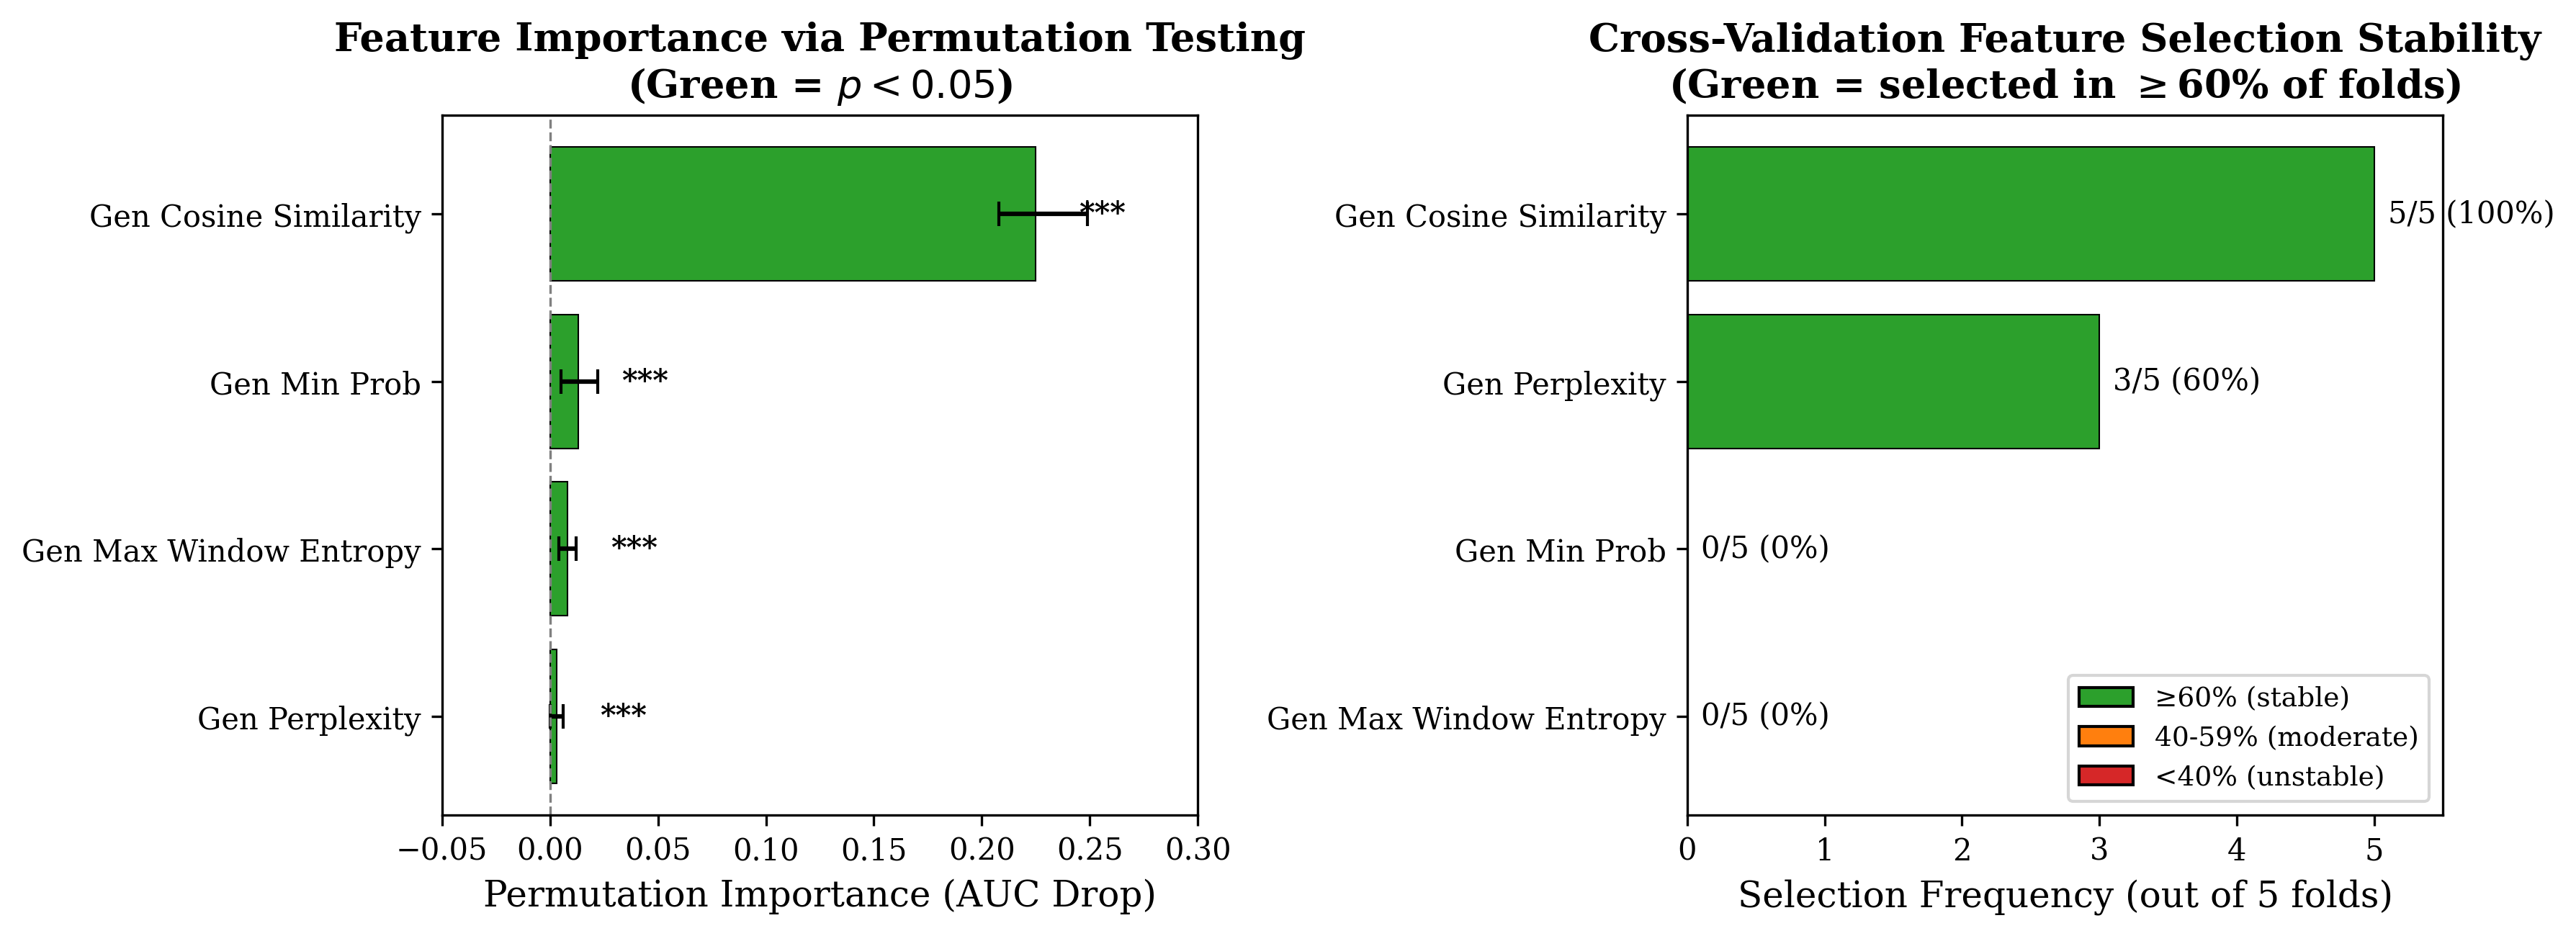
\includegraphics[width=1.0\textwidth]{../../final_runs/RQ2_hallucination_detection/rfe_clean_figure.png}
\caption{Recursive Feature Elimination (RFE) analysis for hallucination detection using Logistic Regression with nested 5$\times$3 cross-validation (unbiased performance estimation). \textbf{Left:} Permutation importance showing contribution of each generator CI metric to classification performance. Statistical significance assessed via one-sample $t$-test (H$_0$: mean AUC drop = 0; one-sided alternative, $n=100$ permutations per feature). Green bars indicate statistically significant features ($p < 0.05$); error bars show 95\% CI from bootstrap percentiles. Gen Cosine Similarity shows highest importance (0.225 AUC drop when permuted). \textbf{Right:} Feature selection stability across 5-fold cross-validation. Colors indicate selection frequency: green ($\geq$60\%), orange (40--59\%), red ($<$40\%). Gen Cosine Similarity was consistently selected (5/5 folds, 100\%); Gen Perplexity was selected in 3/5 folds (60\%). Gen Min Prob and Gen Max Window Entropy were never selected (0/5 folds), indicating they add no predictive value beyond the top two features for Logistic Regression. \textit{Note:} Random Forest (used in Phases 5--6) selected all 4 features due to its higher model capacity, achieving higher in-distribution AUC but poorer cross-domain generalization (Table~\ref{tab:rq2_ensemble_performance}).}
\label{fig:rq2_rfe}
\end{figure}

\subsection{Ensemble Classification Results}

Table~\ref{tab:rq2_ensemble_performance} presents a cross-phase validation analysis designed to detect overfitting. Each phase uses a progressively stricter validation strategy: Phase 4 tests feature selection on all pooled data; Phase 5 evaluates on held-out samples from the same distribution; Phase 6 tests generalization to entirely unseen CLDs. Performance drops between phases indicate the degree to which models exploit CLD-specific patterns rather than learning generalizable hallucination signals.

\begin{table}[H]
\centering
\caption{Ensemble Classifier Performance Across Validation Phases (Cross-Phase Overfitting Analysis)}
\label{tab:rq2_ensemble_performance}
\begin{threeparttable}
\begin{tabular}{lcccccc}
\toprule
\textbf{Classifier} & \textbf{Phase 4:} & \textbf{Phase 5:} & \textbf{Phase 5:} & \textbf{Phase 6:} & \textbf{Performance} & \textbf{Interpretation} \\
 & \textbf{RFE CV AUC} & \textbf{CV AUC} & \textbf{Test AUC} & \textbf{Cross-CLD AUC} & \textbf{Drop (5$\rightarrow$6)} & \\
 & \textbf{(95\% CI)} & \textbf{(95\% CI)} & & \textbf{(95\% CI)} & & \\
\midrule
Neural             & N/A & 0.724 & 0.766 & 0.670 & 0.096 & Mild \\
Network            & & [0.714, 0.734] & & [0.493, 0.847] & & overfitting \\
\midrule
Logistic           & 0.706 & 0.688 & 0.707 & 0.664 & 0.043 & Good \\
Regression         & [0.693, 0.720] & [0.676, 0.701] & & [0.425, 0.903] & & generalization \\
\midrule
Gradient           & 0.812 & 0.806 & 0.815 & 0.644 & 0.171 & Moderate \\
Boosting           & [0.796, 0.828] & [0.789, 0.822] & & [0.348, 0.939] & & overfitting \\
\midrule
Random             & 0.988 & 0.974 & 0.987 & 0.630 & 0.357 & Severe \\
Forest             & [0.985, 0.992] & [0.969, 0.980] & & [0.476, 0.784] & & overfitting \\
\bottomrule
\end{tabular}
\begin{tablenotes}
\small
\item \textit{Note.} Cross-phase validation analysis using 63 experiment files (16,507 total edges, 15.2\% hallucinations). 
\textbf{Phase 4 (RFE CV AUC):} 5-fold stratified CV on \textit{all} pooled edges; measures feature selection performance.
\textbf{Phase 5 (CV AUC):} 5-fold stratified CV on training portion only (70\% of data); measures in-distribution performance.
\textbf{Phase 5 (Test AUC):} Single evaluation on held-out test set (30\% of data); validates generalization within same distribution.
\textbf{Phase 6 (Cross-CLD AUC):} Leave-one-CLD-out CV---train on 2 CLDs, test on held-out 3rd CLD, averaged across all 3 CLDs; measures cross-domain generalization.
Phase 4 evaluates all 4 CI metrics via RFE for each classifier; the best-performing classifier (Random Forest) selected all 4 features, which are then used in Phases 5--6. 
95\% CIs: Phase 4 \& 5 based on 5 folds (df=4); Phase 6 based on 3 CLDs (df=2, wider CIs reflect cross-domain uncertainty). 
Performance Drop = Phase 5 Test AUC $-$ Phase 6 Mean AUC. 
Key finding: Random Forest achieves near-perfect in-distribution performance (AUC=0.987) but severe overfitting to CLD-specific patterns (drops to 0.630 cross-domain). 
Neural Network shows best cross-domain generalization despite lower in-distribution performance.
\end{tablenotes}
\end{threeparttable}
\end{table}

\subsection{Feature Distributions: Correct vs. Hallucinations}

\begin{figure}[H]
\centering
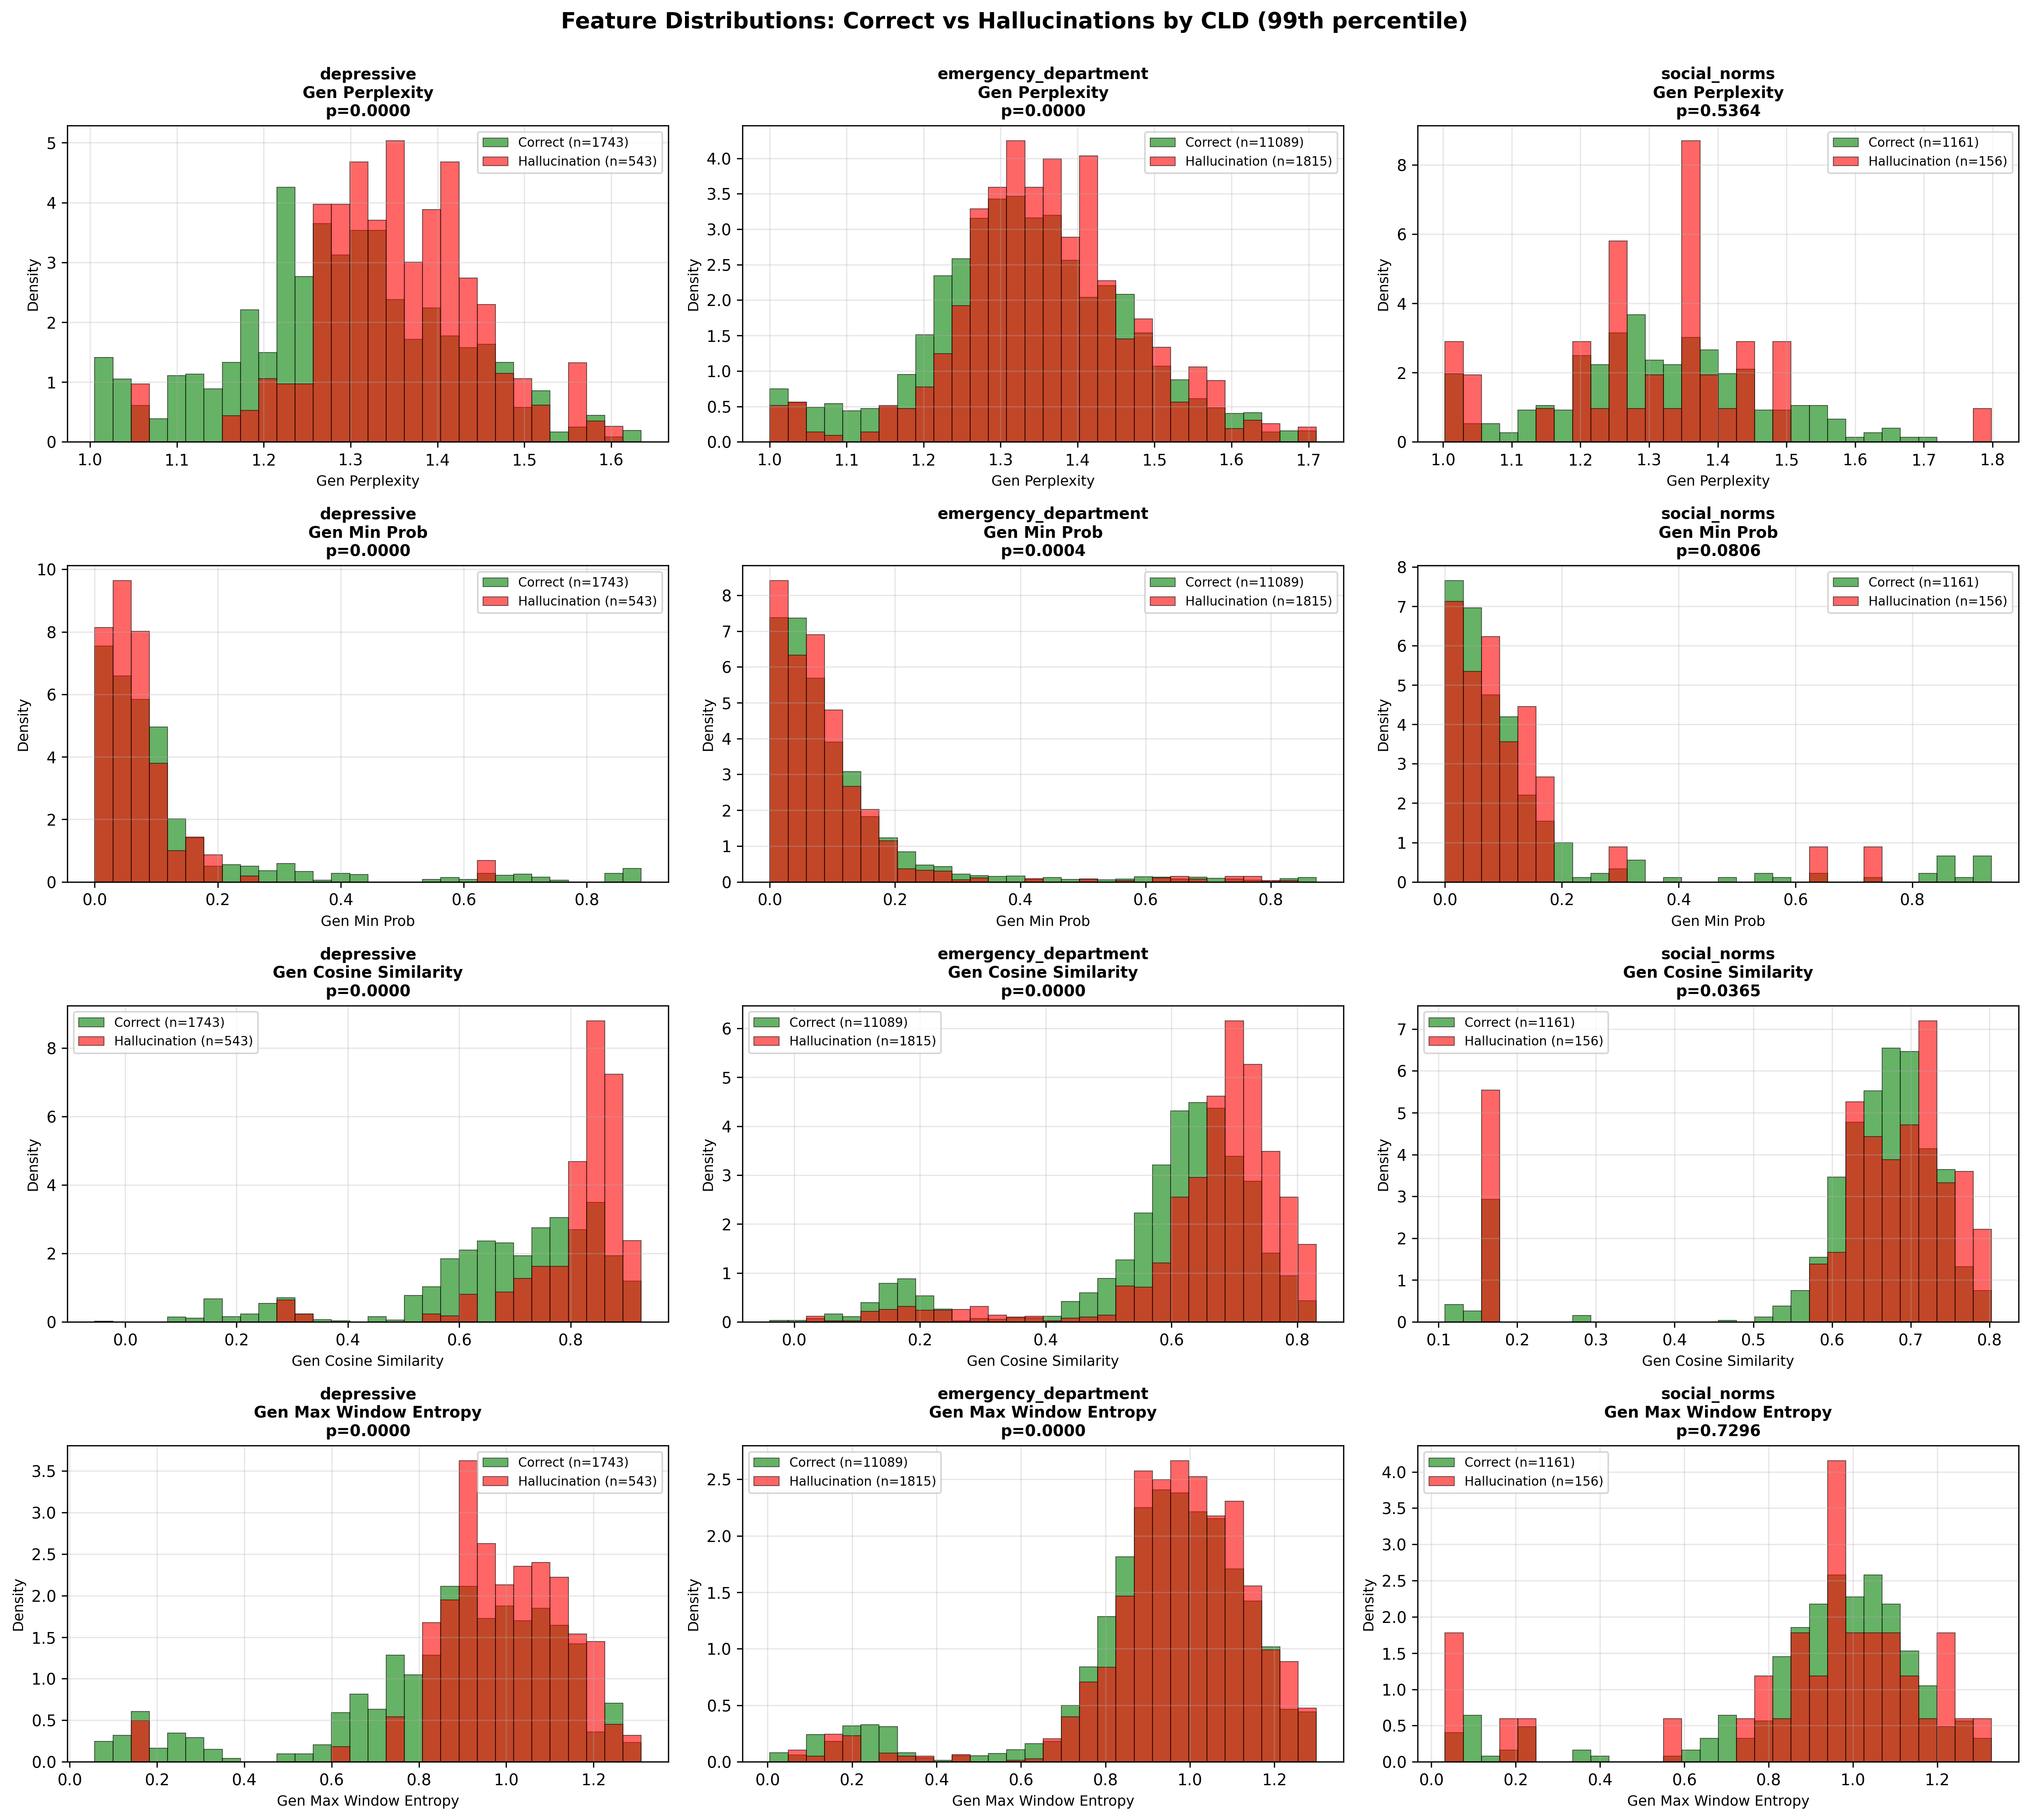
\includegraphics[width=1.0\textwidth]{../../final_runs/RQ2_hallucination_detection/feature_distributions_by_cld_4x3.png}
\caption{Generator CI metric distributions comparing correct edges (green) vs. hallucinations (red) for each CLD (99th percentile). 4×3 grid layout: each row shows one of the 4 generator metrics (Perplexity, Min Prob, Max Window Entropy, Cosine Similarity), with columns representing the three CLDs (Depressive symptoms, Emergency department, Social norms). Statistical significance assessed via Mann-Whitney U test comparing correct vs. hallucination distributions (p-values shown in each subplot). Note the domain-specific variation in metric distributions, particularly for Emergency department which shows the clearest separation, explaining why cross-domain generalization is challenging.}
\label{fig:rq2_distributions_by_cld}
\end{figure}

% ==============================================================================
\section{Prompt Sensitivity Analysis}
% ==============================================================================

To quantify how prompt engineering choices affect judge performance, we perform a sensitivity analysis measuring the relationship between prompt variation (input) and F1 change (output). Prompts are embedded using MPNet~\cite{reimers2019sentencebert}, and cosine distance from the baseline prompt serves as the quantitative input measure. One-way ANOVA tests whether prompt choice significantly affects performance across CLDs and runs.

\begin{figure}[H]
\centering
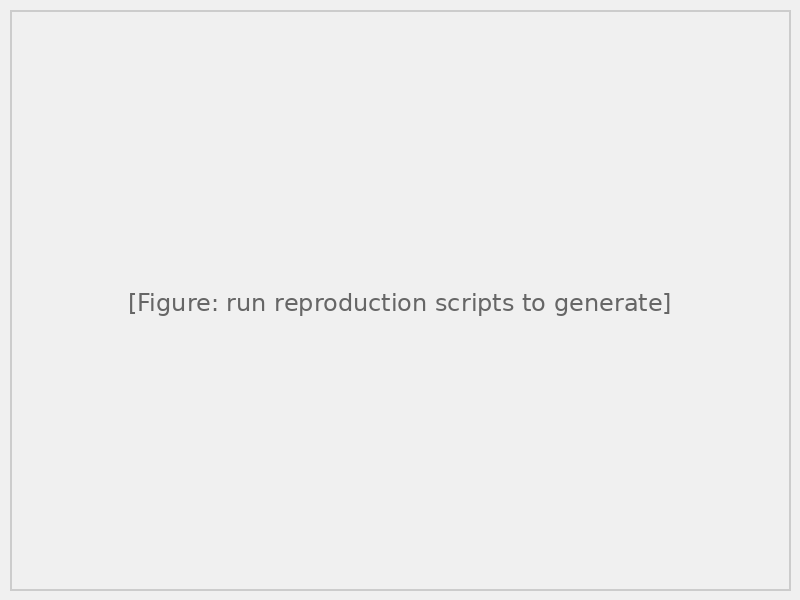
\includegraphics[width=1.0\textwidth]{../../final_runs/Sensitivity_analysis_simple/prompt_sensitivity_figure.png}
\caption{Prompt sensitivity analysis across RQ1a experiments. Each panel shows F1 performance (mean $\pm$ std across CLDs and runs) for prompt variants: Baseline, Chain-of-Thought, Mechanistic, and Mechanistic-Lit (citation only). Statistical test: one-way ANOVA ($\alpha=0.05$); * $p<0.05$, ** $p<0.01$, *** $p<0.001$. Key findings: (1) Correctness judges show significant prompt sensitivity---Corruption Detection ($p=0.020$*) where Mechanistic underperforms, and Ground Truth ($p<0.001$***) where Mechanistic outperforms baseline (+0.24 $\Delta$F1). (2) Citation judges are robust to prompt choice across all 4 variants ($p>0.8$, ns). Dashed lines indicate baseline.}
\label{fig:sensitivity_analysis}
\end{figure}

\begin{table}[H]
\centering
\caption{Prompt Sensitivity Analysis: Performance by Prompt Type Across Experiments}
\label{tab:prompt_sensitivity}
\begin{threeparttable}
\begin{tabular}{llcccccc}
\toprule
\textbf{Experiment} & \textbf{Prompt} & \textbf{Distance} & \textbf{F1} & \textbf{F1 Std} & \textbf{$\Delta$F1} & \textbf{ANOVA p} & \textbf{$\eta^2$} \\
\midrule
Corruption Citation & Baseline & 0.000 & 0.411 & 0.037 & +0.000 & 0.835 & 0.01 \\
 & CoT & 0.019 & 0.411 & 0.035 & +0.000 &  & \\
 & Mechanistic & 0.316 & 0.414 & 0.036 & +0.003 &  & \\
 & Mech\_Lit & 0.318 & 0.415 & 0.036 & +0.004 &  & \\
\midrule
Corruption Correctness & Baseline & 0.000 & 0.786 & 0.036 & +0.000 & 0.007** & 0.48 \\
 & CoT & 0.012 & 0.806 & 0.024 & +0.020 &  & \\
 & Mechanistic & 0.184 & 0.746 & 0.014 & $-$0.040 &  & \\
\midrule
Ground Truth Citation & Baseline & 0.000 & 0.299 & 0.083 & +0.000 & 0.918 & 0.00 \\
 & CoT & 0.019 & 0.284 & 0.086 & $-$0.015 &  & \\
 & Mechanistic & 0.316 & 0.288 & 0.077 & $-$0.011 &  & \\
\midrule
Ground Truth Correctness & Baseline & 0.000 & 0.206 & 0.076 & +0.000 & $<$0.001*** & 0.59 \\
 & CoT & 0.012 & 0.235 & 0.063 & +0.029 &  & \\
 & Mechanistic & 0.184 & 0.447 & 0.120 & +0.241 &  & \\
\bottomrule
\end{tabular}
\begin{tablenotes}
\small
\item \textit{Note.} Statistical test: one-way ANOVA ($\alpha=0.05$). Distance = MPNet cosine distance from baseline. F1 Std = standard deviation across CLDs and runs. $\Delta$F1 = change from baseline.
\item $\eta^2$ = eta-squared effect size: $<$0.06 small, 0.06--0.14 medium, $>$0.14 large.
\item Significance: * $p<0.05$, ** $p<0.01$, *** $p<0.001$; unmarked = not significant.
\item \textit{Assumptions:} Shapiro-Wilk normality and Levene's homogeneity tested per experiment. GT Correctness: all assumptions met. Other experiments: partial violations (Corr.\ Citation: Mechanistic non-normal, $p$=.036; Corr.\ Correctness: unequal variances, Levene $p$=.004; GT Citation: non-normal distributions). Results robust: non-significant findings remain non-significant under Kruskal-Wallis; GT Correctness significant finding ($p<.001$) met all assumptions.
\item \textit{Multiple comparisons:} Bonferroni-corrected for 4 tests within RQ1a ($\alpha_{\text{adj}} = 0.0125$). Adjusted $p$-values: Corr.\ Correctness $p_{\text{adj}}=.028$*, GT Correctness $p_{\text{adj}}=.004$**. Both remain significant after correction.
\item Key finding: Prompt choice significantly affects correctness judges (large effect, $\eta^2 = 0.48$--$0.59$) but not citation judges (negligible effect, $\eta^2 \leq 0.01$).
\end{tablenotes}
\end{threeparttable}
\end{table}

% ==============================================================================
\section{Corrector Prompt Sensitivity Analysis}
% ==============================================================================

Extending the sensitivity analysis to the LLM-as-a-Corrector (RQ1b), we evaluate how corrector prompt complexity affects correction performance. Unlike judge prompts which had distinct semantic content, corrector prompts follow a cumulative design: Baseline provides examples only, CoT adds step-by-step reasoning (1.45$\times$ length), and Mechanistic adds Bradford Hill criteria (1.91$\times$ length).

\begin{figure}[H]
\centering
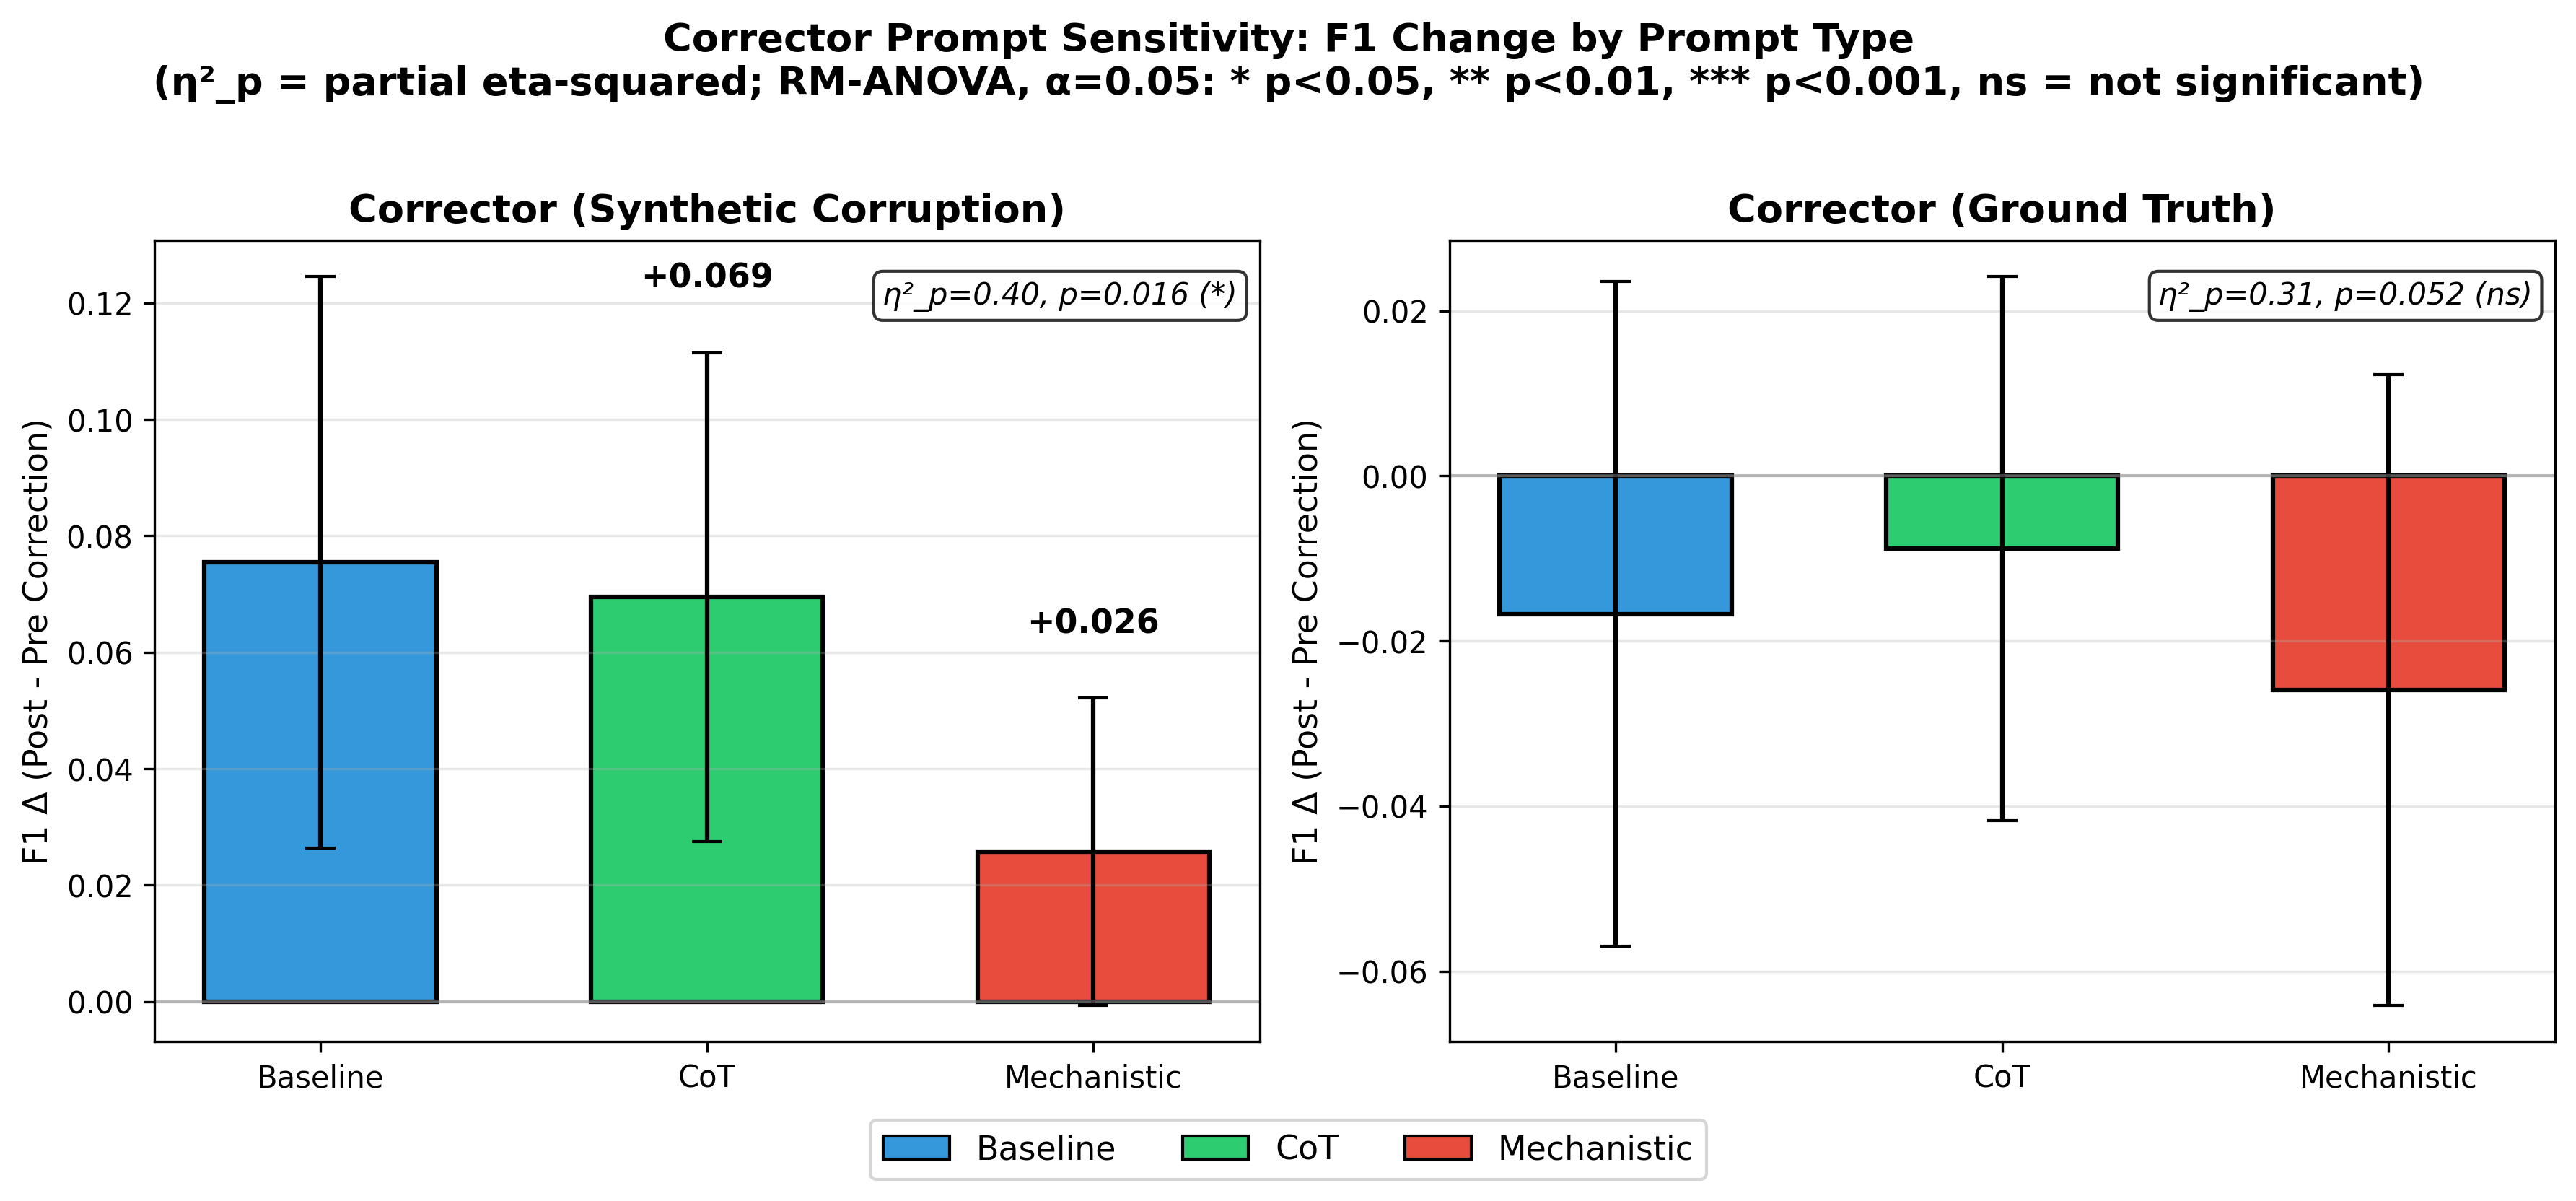
\includegraphics[width=1.0\textwidth]{../../final_runs/Sensitivity_analysis_simple/corrector_sensitivity_figure.png}
\caption{Corrector prompt sensitivity analysis. F1 $\Delta$ (post-correction minus pre-correction) by prompt type. Statistical test: one-way ANOVA ($\alpha=0.05$). Error bars show standard deviation across CLDs and runs. Neither experiment shows significant prompt sensitivity: Synthetic ($p=0.166$, ns), Ground Truth ($p=0.372$, ns). Key finding: Simpler prompts (Baseline: +0.075) show better mean correction than complex prompts (Mechanistic: +0.026), though not statistically significant.}
\label{fig:corrector_sensitivity}
\end{figure}

\begin{table}[H]
\centering
\caption{Corrector Prompt Sensitivity Analysis: F1 Change by Prompt Type}
\label{tab:corrector_sensitivity}
\begin{threeparttable}
\begin{tabular}{llccccccc}
\toprule
\textbf{Experiment} & \textbf{Prompt} & \textbf{Distance} & \textbf{Length} & \textbf{F1 $\Delta$} & \textbf{Std} & \textbf{N} & \textbf{ANOVA p} & \textbf{$\eta^2$} \\
\midrule
Synthetic & Baseline & 0.000 & 1.00$\times$ & +0.075 & 0.060 & 9 & 0.166 & 0.14 \\
 & CoT & 0.000 & 1.45$\times$ & +0.063 & 0.060 & 9 &  & \\
 & Mechanistic & 0.000 & 1.91$\times$ & +0.026 & 0.032 & 9 &  & \\
\midrule
Ground Truth & Baseline & 0.000 & 1.00$\times$ & $-$0.017 & 0.049 & 9 & 0.372 & 0.10 \\
 & CoT & 0.000 & 1.45$\times$ & +0.026 & 0.003 & 3 &  & \\
 & Mechanistic & 0.000 & 1.91$\times$ & $-$0.016 & 0.043 & 9 &  & \\
\bottomrule
\end{tabular}
\begin{tablenotes}
\small
\item \textit{Note.} Statistical test: one-way ANOVA ($\alpha=0.05$). Distance = Jina v2 cosine distance from baseline (8192-token context). Length = prompt length ratio (cumulative design). F1 $\Delta$ = change from pre- to post-correction.
\item $\eta^2$ = eta-squared effect size: $<$0.06 small, 0.06--0.14 medium, $>$0.14 large.
\item Significance: * $p<0.05$, ** $p<0.01$; unmarked = not significant ($p>0.05$).
\item \textit{Assumptions:} Shapiro-Wilk normality and Levene's homogeneity tested. Ground Truth: all assumptions met. Synthetic: normality violated for CoT ($p$=.024) and Mechanistic ($p$=.011); homogeneity OK (Levene $p$=.089). Non-significance robust: Kruskal-Wallis yields same conclusion.
\item Key finding: Simpler prompts (Baseline: +0.075) outperform complex prompts (Mechanistic: +0.026) with medium-large effect size ($\eta^2 = 0.14$), though not statistically significant due to high variance.
\end{tablenotes}
\end{threeparttable}
\end{table}

% ==============================================================================
\section{RQ3: Deep Research Literature Validation}
% ==============================================================================

\begin{center}
\fbox{\parbox{0.95\textwidth}{
\textbf{Methodological Pivot:} The original RQ3 (smart test-time compute using CI metrics to selectively deploy correctors) was predicated on RQ2 generalization and RQ1b corrector efficacy---conditions not supported by our findings. We pivoted to \textbf{Deep Research validation} as an alternative test-time compute strategy: rather than \textit{correcting} hallucinations, we test whether automated literature search can \textit{validate} causal claims. This is presented as an exploratory pilot study with acknowledged limitations (single-run, no ablation). See Discussion (Section~\ref{sec:rq3_pivot}) for rationale.
}}
\end{center}

\vspace{0.5em}

We deployed the Deep Research (DR) system on 285 edges classified by ground truth validation across all 3 CLDs (Depressive Symptoms, Social Norms, Older Persons) to test whether automated literature search can validate causal claims. The key metric is \textbf{detection rate}: percentage of edges for which DR found \textit{direct causal evidence} (RCTs, experimental manipulations, or meta-analyses---not correlational studies).

\begin{table}[H]
\centering
\caption{Deep Research Detection Rate and Discrimination Analysis (n=285 edges)}
\label{tab:rq3_results}
\begin{threeparttable}
\begin{tabular}{lccccl}
\toprule
\textbf{Classification} & \textbf{n} & \textbf{Detection Rate} & \textbf{Confidence} & \textbf{vs TP Gap} & \textbf{Discrimination} \\
\midrule
TP (Expert-accepted) & 44 & 70.5\% & 7.35 & --- & Reference \\
FP (LLM hallucinations) & 178 & 62.4\% & 7.63 & $-$8.1 pp & \textcolor{red}{\textbf{NOT SIG.}} \\
FN (Expert-rejected) & 63 & 42.9\% & 7.81 & $-$27.6 pp & \textcolor{green}{SIGNIFICANT} \\
\bottomrule
\end{tabular}
\begin{tablenotes}
\small
\item \textit{Note.} Detection rate = \% edges with direct causal evidence found. Confidence = self-assessed (1--10 scale, range = 0.46). TP/FP/FN from RQ1a GT Lit validation across all 3 CLDs.
\item \textit{Assumption testing:} Chi-square assumptions met ($N=222$, all expected cells $\geq 5$, min expected = 15.9).
\item \textit{TP--FP test:} Fisher's exact $p=.38$; OR = 1.44 [95\% CI: 0.70, 2.94]; Cohen's $h=0.17$ [95\% CI: $-$0.16, 0.50] (negligible); achieved power = 17\%.
\item \textit{TP--FN test:} Fisher's exact $p=.006$**; Cohen's $h=0.57$ [95\% CI: 0.18, 0.95] (medium); power = 82\%.
\item \textit{Multiple comparisons:} Bonferroni-corrected for 3 pairwise tests within RQ3 ($\alpha_{\text{adj}} = 0.017$). TP--FN $p_{\text{adj}}=.018$* and FP--FN $p_{\text{adj}}=.024$* remain significant.
\item \textbf{Finding:} TP--FP gap (8.1 pp) is \textit{not} statistically significant ($p=.38$, underpowered). Effect size CI includes zero. TP--FN discrimination \textit{is} significant ($p<.01$, survives correction).
\end{tablenotes}
\end{threeparttable}
\end{table}

\begin{figure}[H]
\centering
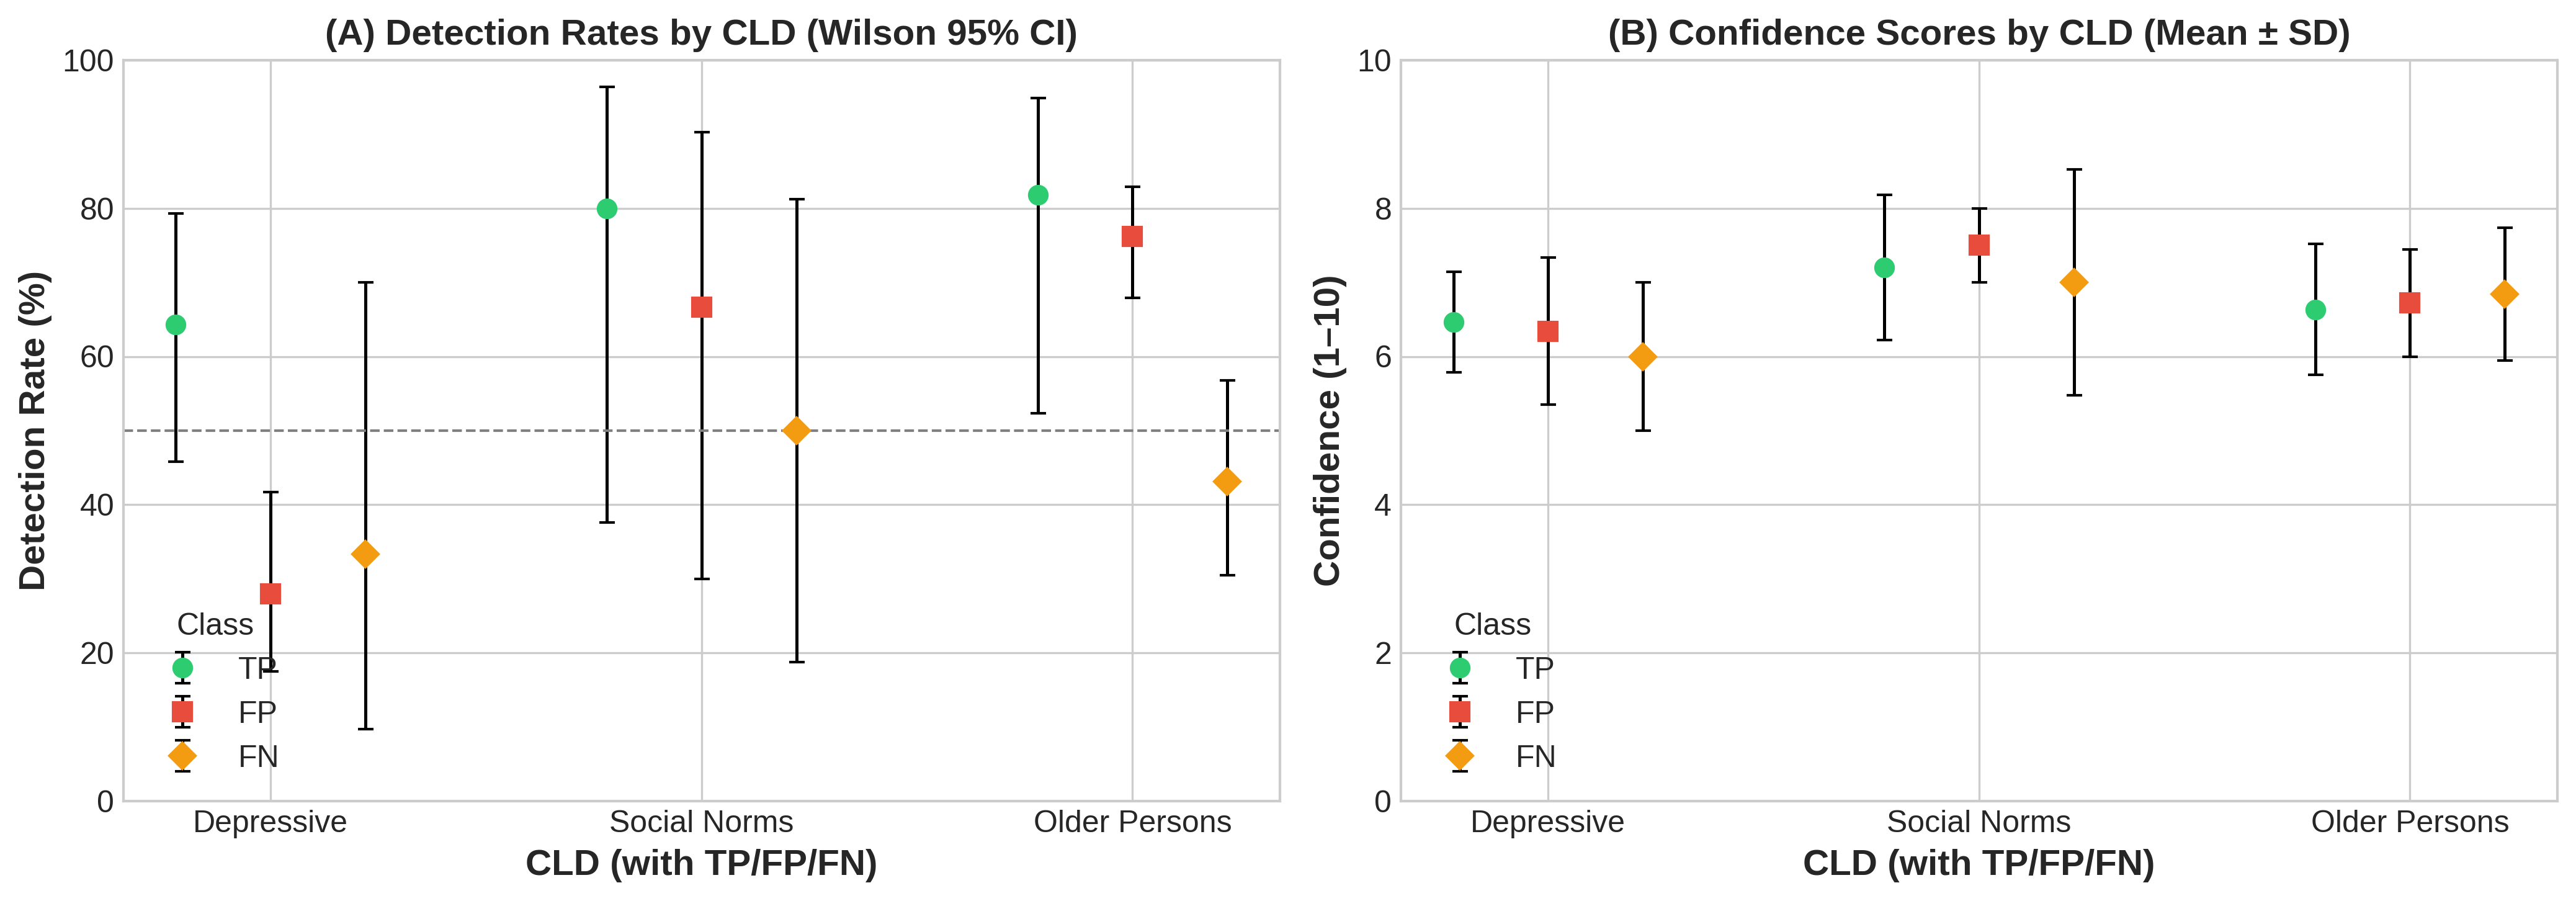
\includegraphics[width=1.0\textwidth]{../../final_runs/RQ3_deep_research/figures/rq3_combined_figure.png}
\caption{Deep Research results. \textbf{(A)} Detection rates: TP (70.5\%) $>$ FP (62.4\%), gap = 8.1 pp (not statistically significant, $p=.38$). \textbf{(B)} Confidence scores show limited discriminative power (range = 0.46 on 10-point scale).}
\label{fig:rq3_combined}
\end{figure}

\textbf{Key Finding:} Deep Research does \textit{not} significantly discriminate between valid and hallucinated causal claims in aggregate (8.1 pp gap, $p=.38$, Cohen's $h=0.17$ negligible). However, 62\% of LLM hallucinations are validated by automated literature search, suggesting many ``false positives'' may represent plausible relationships that experts excluded for scope/theoretical reasons rather than lack of evidence. The FP--FN gap (+19.5 pp, $p=.008$**, $p_{\text{adj}}=.024$*) survives correction: hallucinated edges have \textit{more} literature support than expert-rejected edges.

\textbf{Critical insight:} Aggregate results mask substantial domain variation (Table~\ref{tab:rq3_per_cld}). Depressive CLD shows strong discrimination (TP--FP gap = +36 pp), while Older Persons shows negligible discrimination (+6 pp). This suggests DR's utility is domain-dependent.

\subsection{Per-CLD Detection Rate Analysis}

\begin{table}[H]
\centering
\caption{Deep Research Detection Rates by CLD and Classification}
\label{tab:rq3_per_cld}
\begin{threeparttable}
\begin{tabular}{llcccc}
\toprule
\textbf{CLD} & \textbf{Class} & \textbf{n} & \textbf{Found} & \textbf{Detection Rate} & \textbf{TP--FP Gap} \\
\midrule
Depressive & TP & 28 & 18 & 64.3\% & \textbf{+36.3 pp} \\
 & FP & 50 & 14 & 28.0\% & --- \\
 & FN & 6 & 2 & 33.3\% & --- \\
\midrule
Social Norms & TP & 5 & 4 & 80.0\% & +13.3 pp \\
 & FP & 6 & 4 & 66.7\% & --- \\
 & FN & 6 & 3 & 50.0\% & --- \\
\midrule
Older Persons & TP & 11 & 9 & 81.8\% & +5.6 pp \\
 & FP & 122 & 93 & 76.2\% & --- \\
 & FN & 51 & 22 & 43.1\% & --- \\
\midrule
\textit{Aggregate} & TP & 44 & 31 & 70.5\% & +8.1 pp \\
 & FP & 178 & 111 & 62.4\% & --- \\
 & FN & 63 & 27 & 42.9\% & --- \\
\bottomrule
\end{tabular}
\begin{tablenotes}
\small
\item \textit{Note.} Detection Rate = percentage of edges where Deep Research found direct causal evidence.
\item TP = True Positives (expert-accepted), FP = False Positives (LLM hallucinations), FN = False Negatives (expert-included but LLM-missed).
\item \textbf{Key finding:} FP detection rate varies substantially by CLD (28\%--76\%), a 48 pp spread. Depressive shows lowest FP detection (28\%) and strongest TP--FP discrimination (+36 pp); Older Persons shows highest FP detection (76\%) and weakest discrimination (+6 pp).
\item \textit{Interpretation:} In the Depressive domain, DR can meaningfully distinguish valid from hallucinated edges; in Older Persons, DR validates most edges regardless of ground truth status.
\end{tablenotes}
\end{threeparttable}
\end{table}

\subsection{Exploratory: Ground Truth Enrichment Analysis}
\label{sec:gt_enrichment_results}

Given that 62.4\% of FP edges have literature support, we explore what LLM generation metrics would be if these DR-validated ``hallucinations'' were reclassified as valid edges---i.e., if we enriched the expert ground truth with literature-supported relationships experts omitted.

\begin{table}[H]
\centering
\caption{LLM Generation Metrics: Two Enrichment Scenarios (Aggregate and Per-CLD)}
\label{tab:enriched_gt}
\begin{threeparttable}
\footnotesize
\begin{tabular}{lccccccc}
\toprule
& \textbf{Original} & \multicolumn{2}{c}{\textbf{Scenario 1: Enriched GT}} & \multicolumn{2}{c}{\textbf{Scenario 2: LLM+DR System}} \\
\cmidrule(lr){3-4} \cmidrule(lr){5-6}
\textbf{Dataset} & \textbf{F1} & \textbf{F1} & \textbf{FPs $\to$ TP} & \textbf{F1} & \textbf{FNs found} \\
\midrule
\textbf{Aggregate} & 0.267 & 0.705 (+163\%) & 111/178 (62\%) & 0.779 (+191\%) & 27/63 (43\%) \\
\midrule
Depressive & 0.500 & 0.667 (+33\%) & 14/50 (28\%) & 0.687 (+37\%) & 2/6 (33\%) \\
Social Norms & 0.455 & 0.692 (+52\%) & 4/6 (67\%) & 0.828 (+82\%) & 3/6 (50\%) \\
Older Persons & 0.113 & 0.722 (+539\%) & 93/122 (76\%) & 0.813 (+619\%) & 22/51 (43\%) \\
\bottomrule
\end{tabular}
\begin{tablenotes}
\small
\item \textit{Scenario 1 (Enriched GT):} Promotes FP edges with DR evidence to TP. Tests: ``What if experts missed valid relationships?''
\item \textit{Scenario 2 (LLM+DR System):} Scenario 1 + DR discovers FN edges with literature support. Tests: ``What could a complete LLM+DR pipeline achieve?''
\item \textit{Aggregate confusion matrices:} Original: TP=44, FP=178, FN=63. Scenario 1: TP=155, FP=67, FN=63. Scenario 2: TP=182, FP=67, FN=36.
\end{tablenotes}
\end{threeparttable}
\end{table}

\textbf{FN Analysis (Scenario 2):} Of 63 FN edges (expert-included, LLM-missed): 27 (42.9\%) have DR evidence---in a complete LLM+DR system, these would be discovered via literature search and added to the output, reducing FN to 36. The remaining 36 edges (57.1\%) lack searchable evidence, suggesting tacit clinical knowledge or experience not represented in indexed literature.

\textbf{Interpretation:} Scenario 1 asks ``what if experts missed valid relationships?'' (F1: $0.267 \to 0.705$). Scenario 2 asks ``what could a complete LLM+DR pipeline achieve?'' (F1: $0.267 \to 0.779$). The 36 residual FNs represent the irreducible gap---expert knowledge that neither LLM generation nor literature search can recover.

\begin{center}
\fbox{\parbox{0.92\textwidth}{
\textbf{Critical Caveats:} Both scenarios are \textbf{exploratory and preliminary}. Key limitations: (1) DR may validate correlational rather than causal evidence; (2) domain variation is extreme (28\% vs 76\% FP promotion); (3) LLM-based DR validating LLM-generated edges risks circularity; (4) no expert review of promoted/discovered edges; (5) \textbf{True Negatives not analyzed}---DR covered only 20.4\% of the edge space (285 of 1,394 possible edges); the 1,109 TN edges were not analyzed due to cost (\$0.87/edge, \$269 for all TNs). These metrics represent \textbf{upper bounds} on achievable performance, pending domain expert validation. Dataset available for community verification (see Data Availability).
}}
\end{center}

% ==============================================================================
\section{Effect Size Summary}
% ==============================================================================

Table~\ref{tab:effect_sizes} summarizes the standardized effect sizes observed across all research questions, linking each finding to its stated hypothesis and statistical significance. This provides a unified view of which hypotheses were supported and the magnitude of effects detected.

\begin{table}[H]
\centering
\caption{Effect Size Summary with Hypotheses, Significance, and Conclusions}
\label{tab:effect_sizes}
\begin{threeparttable}
\scriptsize
\begin{tabular}{llllcccc}
\toprule
\textbf{RQ} & \textbf{Hypothesis} & \textbf{Comparison} & \textbf{Metric} & \textbf{Effect} & \textbf{Value} & \textbf{$p$} & \textbf{Conclusion} \\
\midrule
1a & Prompt affects F1 & Corr. Citation & F1 & $f$ & 0.10 & .835 & Robust \\
   &                   & Corr. Correctness & F1 & $f$ & 0.96 & .007** & Sensitive \\
   &                   & GT Citation & F1 & $f$ & 0.00 & .918 & Robust \\
   &                   & GT Correctness & F1 & $f$ & 1.20 & $<$.001*** & Sensitive \\
\midrule
1b & Corrector improves CLD & Synth. Baseline & $\Delta$F1 & $d$ & +1.25 & $<$.05* & Effective \\
   &                        & GT Baseline & $\Delta$F1 & $d$ & $-$0.35 & .12 & Ineffective \\
\midrule
2 & CI predicts halluc. & Cosine vs halluc. & AUC & $r$ & 0.152 & $<$.001*** & Weak signal \\
  &                     & Phase 5$\to$6 drop & AUC & $\Delta$ & 0.357 & — & Poor gen. \\
\midrule
3 & DR discriminates TP/FP & TP--FP gap & Prop. & $h$ & 0.17 & .38 & No discrim. \\
\bottomrule
\end{tabular}
\begin{tablenotes}
\scriptsize
\item \textit{Note.} Effect sizes (Cohen, 1988): $f$/$d$/$h$: $<$0.2 negl., 0.2--0.5 small, 0.5--0.8 med., $\geq$0.8 large. $r$: $<$0.1 negl., 0.1--0.3 small, 0.3--0.5 med., $\geq$0.5 large.
\item Significance: * $p<.05$, ** $p<.01$, *** $p<.001$. RQ1a $p$-values from one-way ANOVA (Table~\ref{tab:prompt_sensitivity}).
\item \textit{Multiple comparisons:} Bonferroni correction applied within each RQ family. All significant findings ($p<.05$) survive correction. See Methods \S4.5.
\item \textbf{Summary:} RQ1a---Citation robust to prompt ($p>.8$); correctness sensitive ($p<.01$, survives correction). RQ1b---Corrector effective on synthetic (+1.25$d$) but not GT. RQ2---Weak discrimination ($r$=0.15), poor cross-CLD generalization ($\Delta$AUC=0.36). RQ3---Negligible TP--FP discrimination ($h$=0.17, 95\% CI includes 0, power=17\%).
\end{tablenotes}
\end{threeparttable}
\end{table}

% ==============================================================================
\section{Computational Scaling Analysis}
% ==============================================================================

\subsection{Time and Cost Scaling}

\begin{figure}[H]
\centering
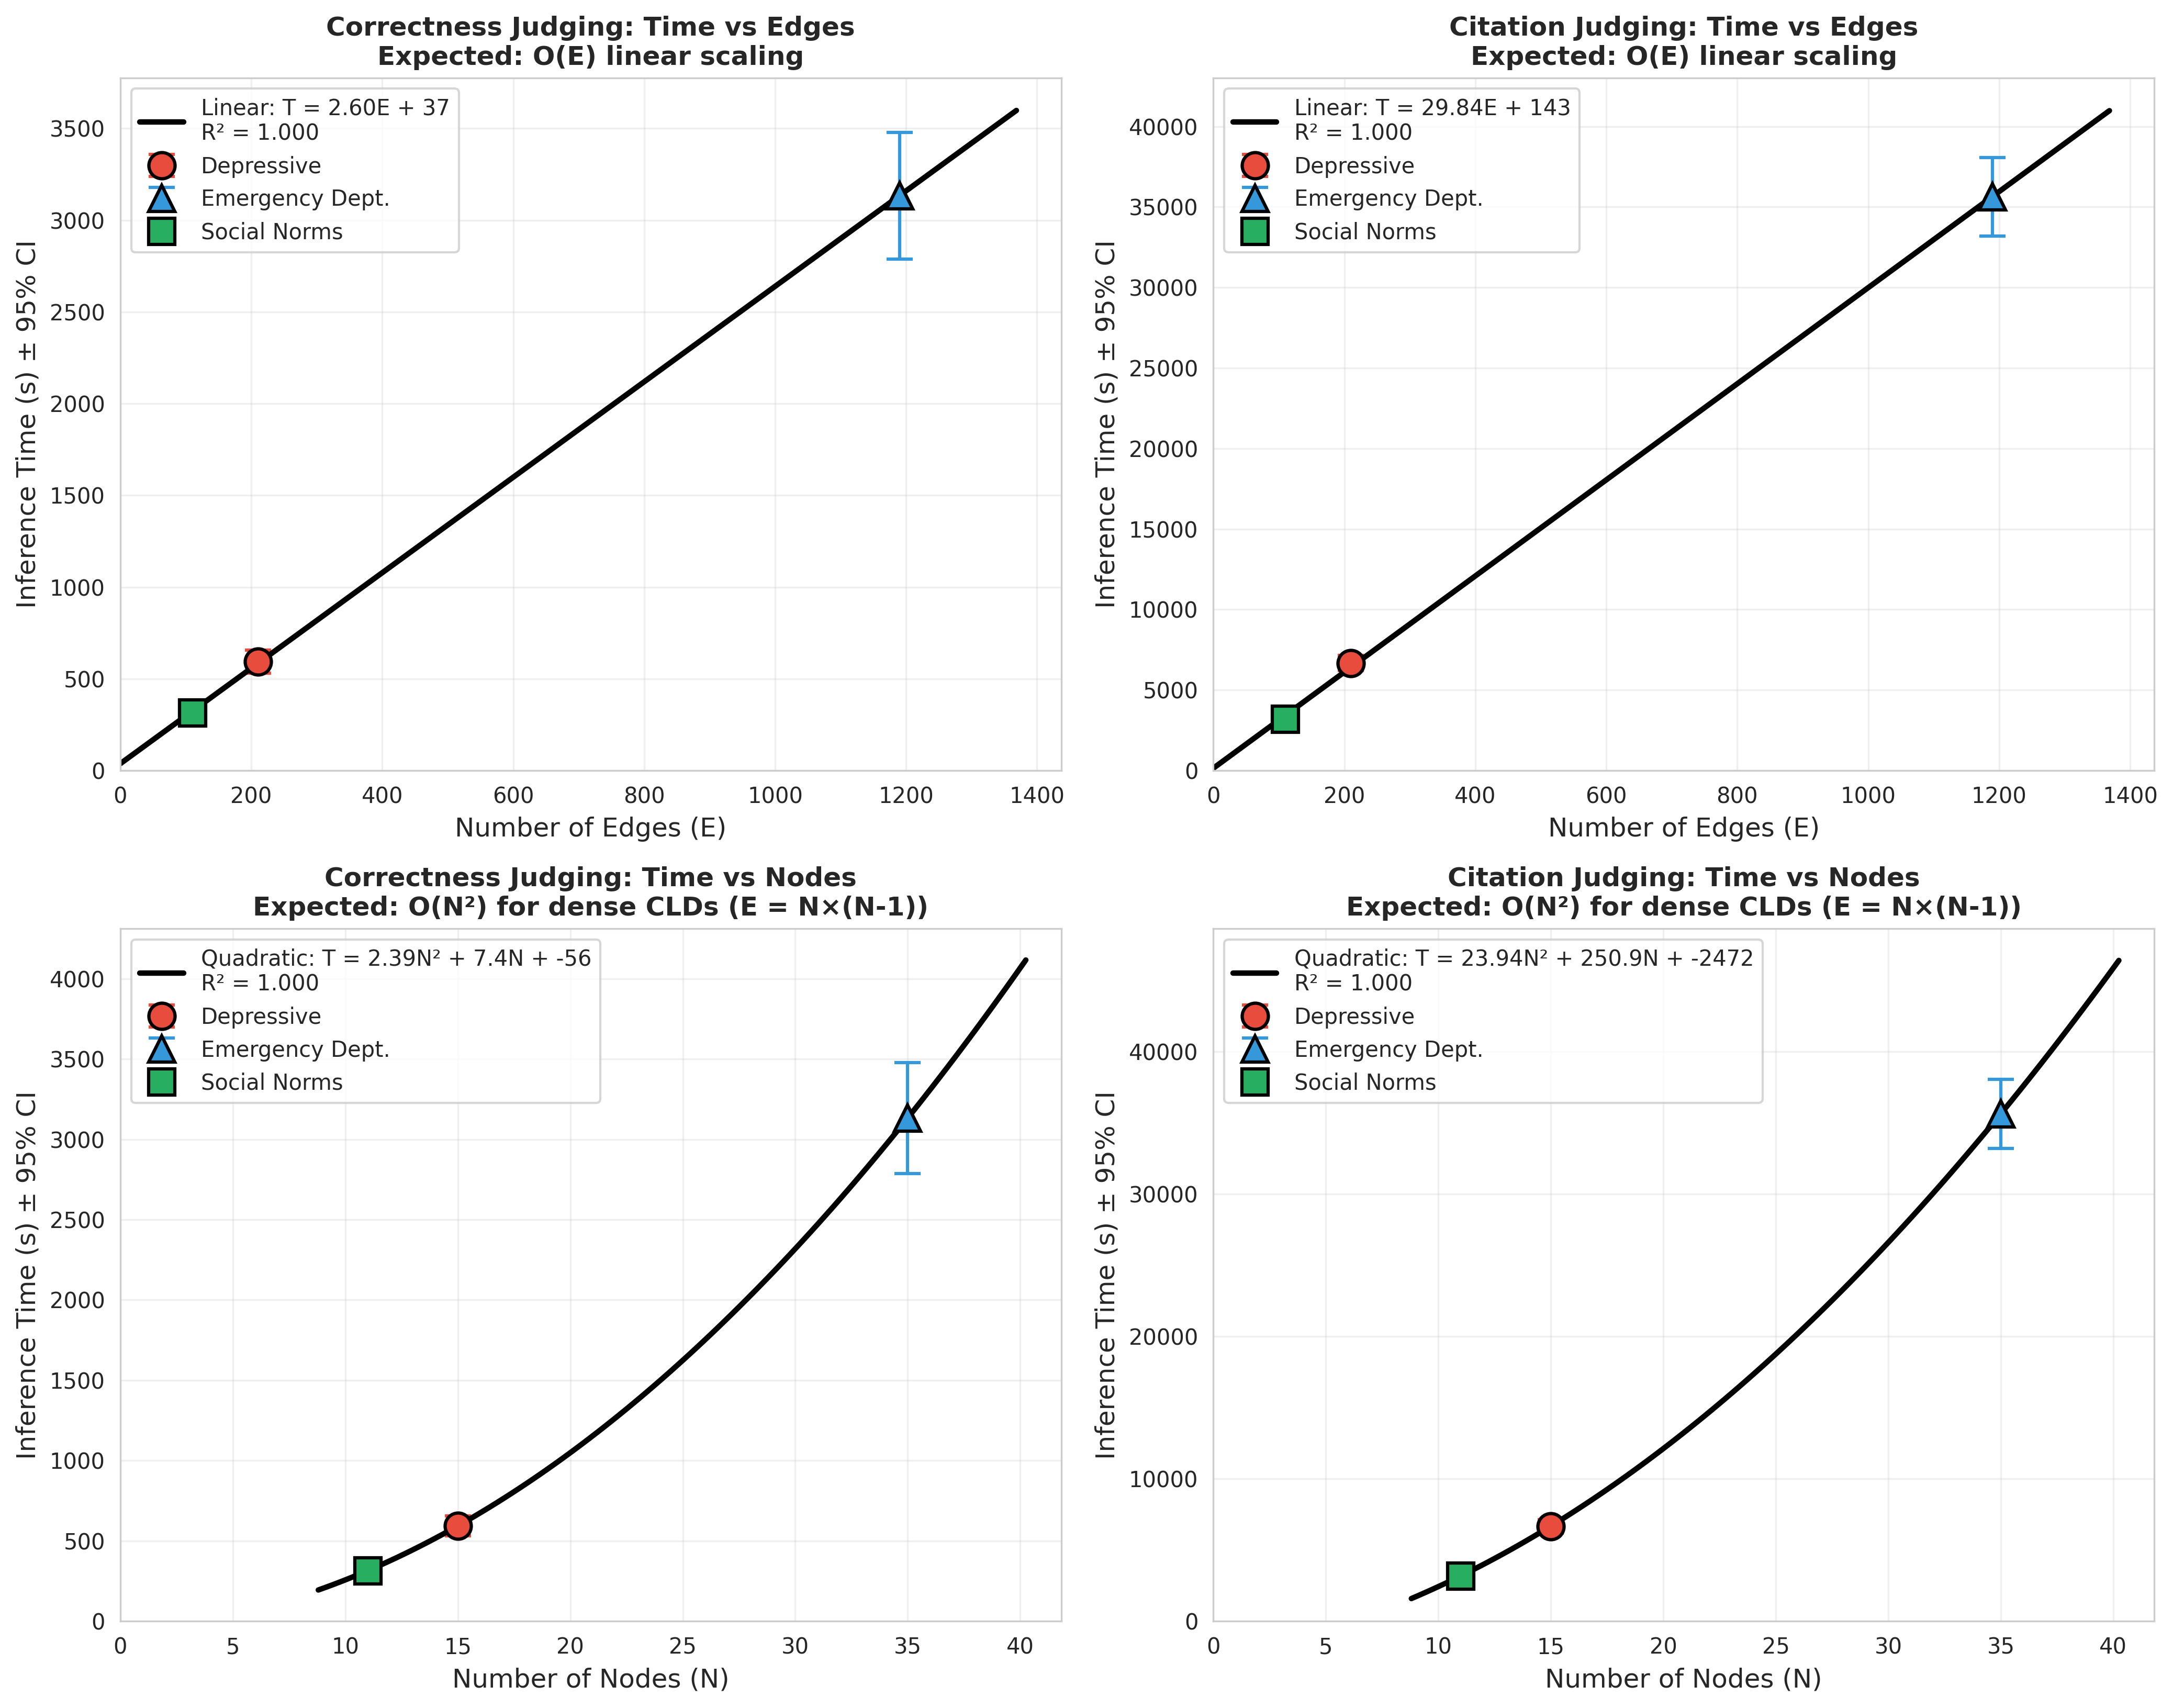
\includegraphics[width=1.0\textwidth]{../../final_runs/time_and_cost_scaling/figures/figure1_scaling_analysis.png}
\caption{Time scaling analysis for CLD judging. \textbf{Top row:} Time vs. number of edges shows linear $O(E)$ scaling. \textbf{Bottom row:} Time vs. number of nodes shows quadratic $O(N^2)$ scaling, consistent with dense CLD structure where $E \approx N(N-1)$. Citation judging (right) is $\sim$11$\times$ slower than correctness (left) due to web search and document retrieval. Points represent per-CLD means $\pm$ 95\% CI (error bars); regression lines show fitted models with $R^2$ values. All three CLDs shown: Depressive (D), Social Norms (S), Emergency Department (E).}
\label{fig:scaling_analysis}
\end{figure}

\begin{figure}[H]
\centering
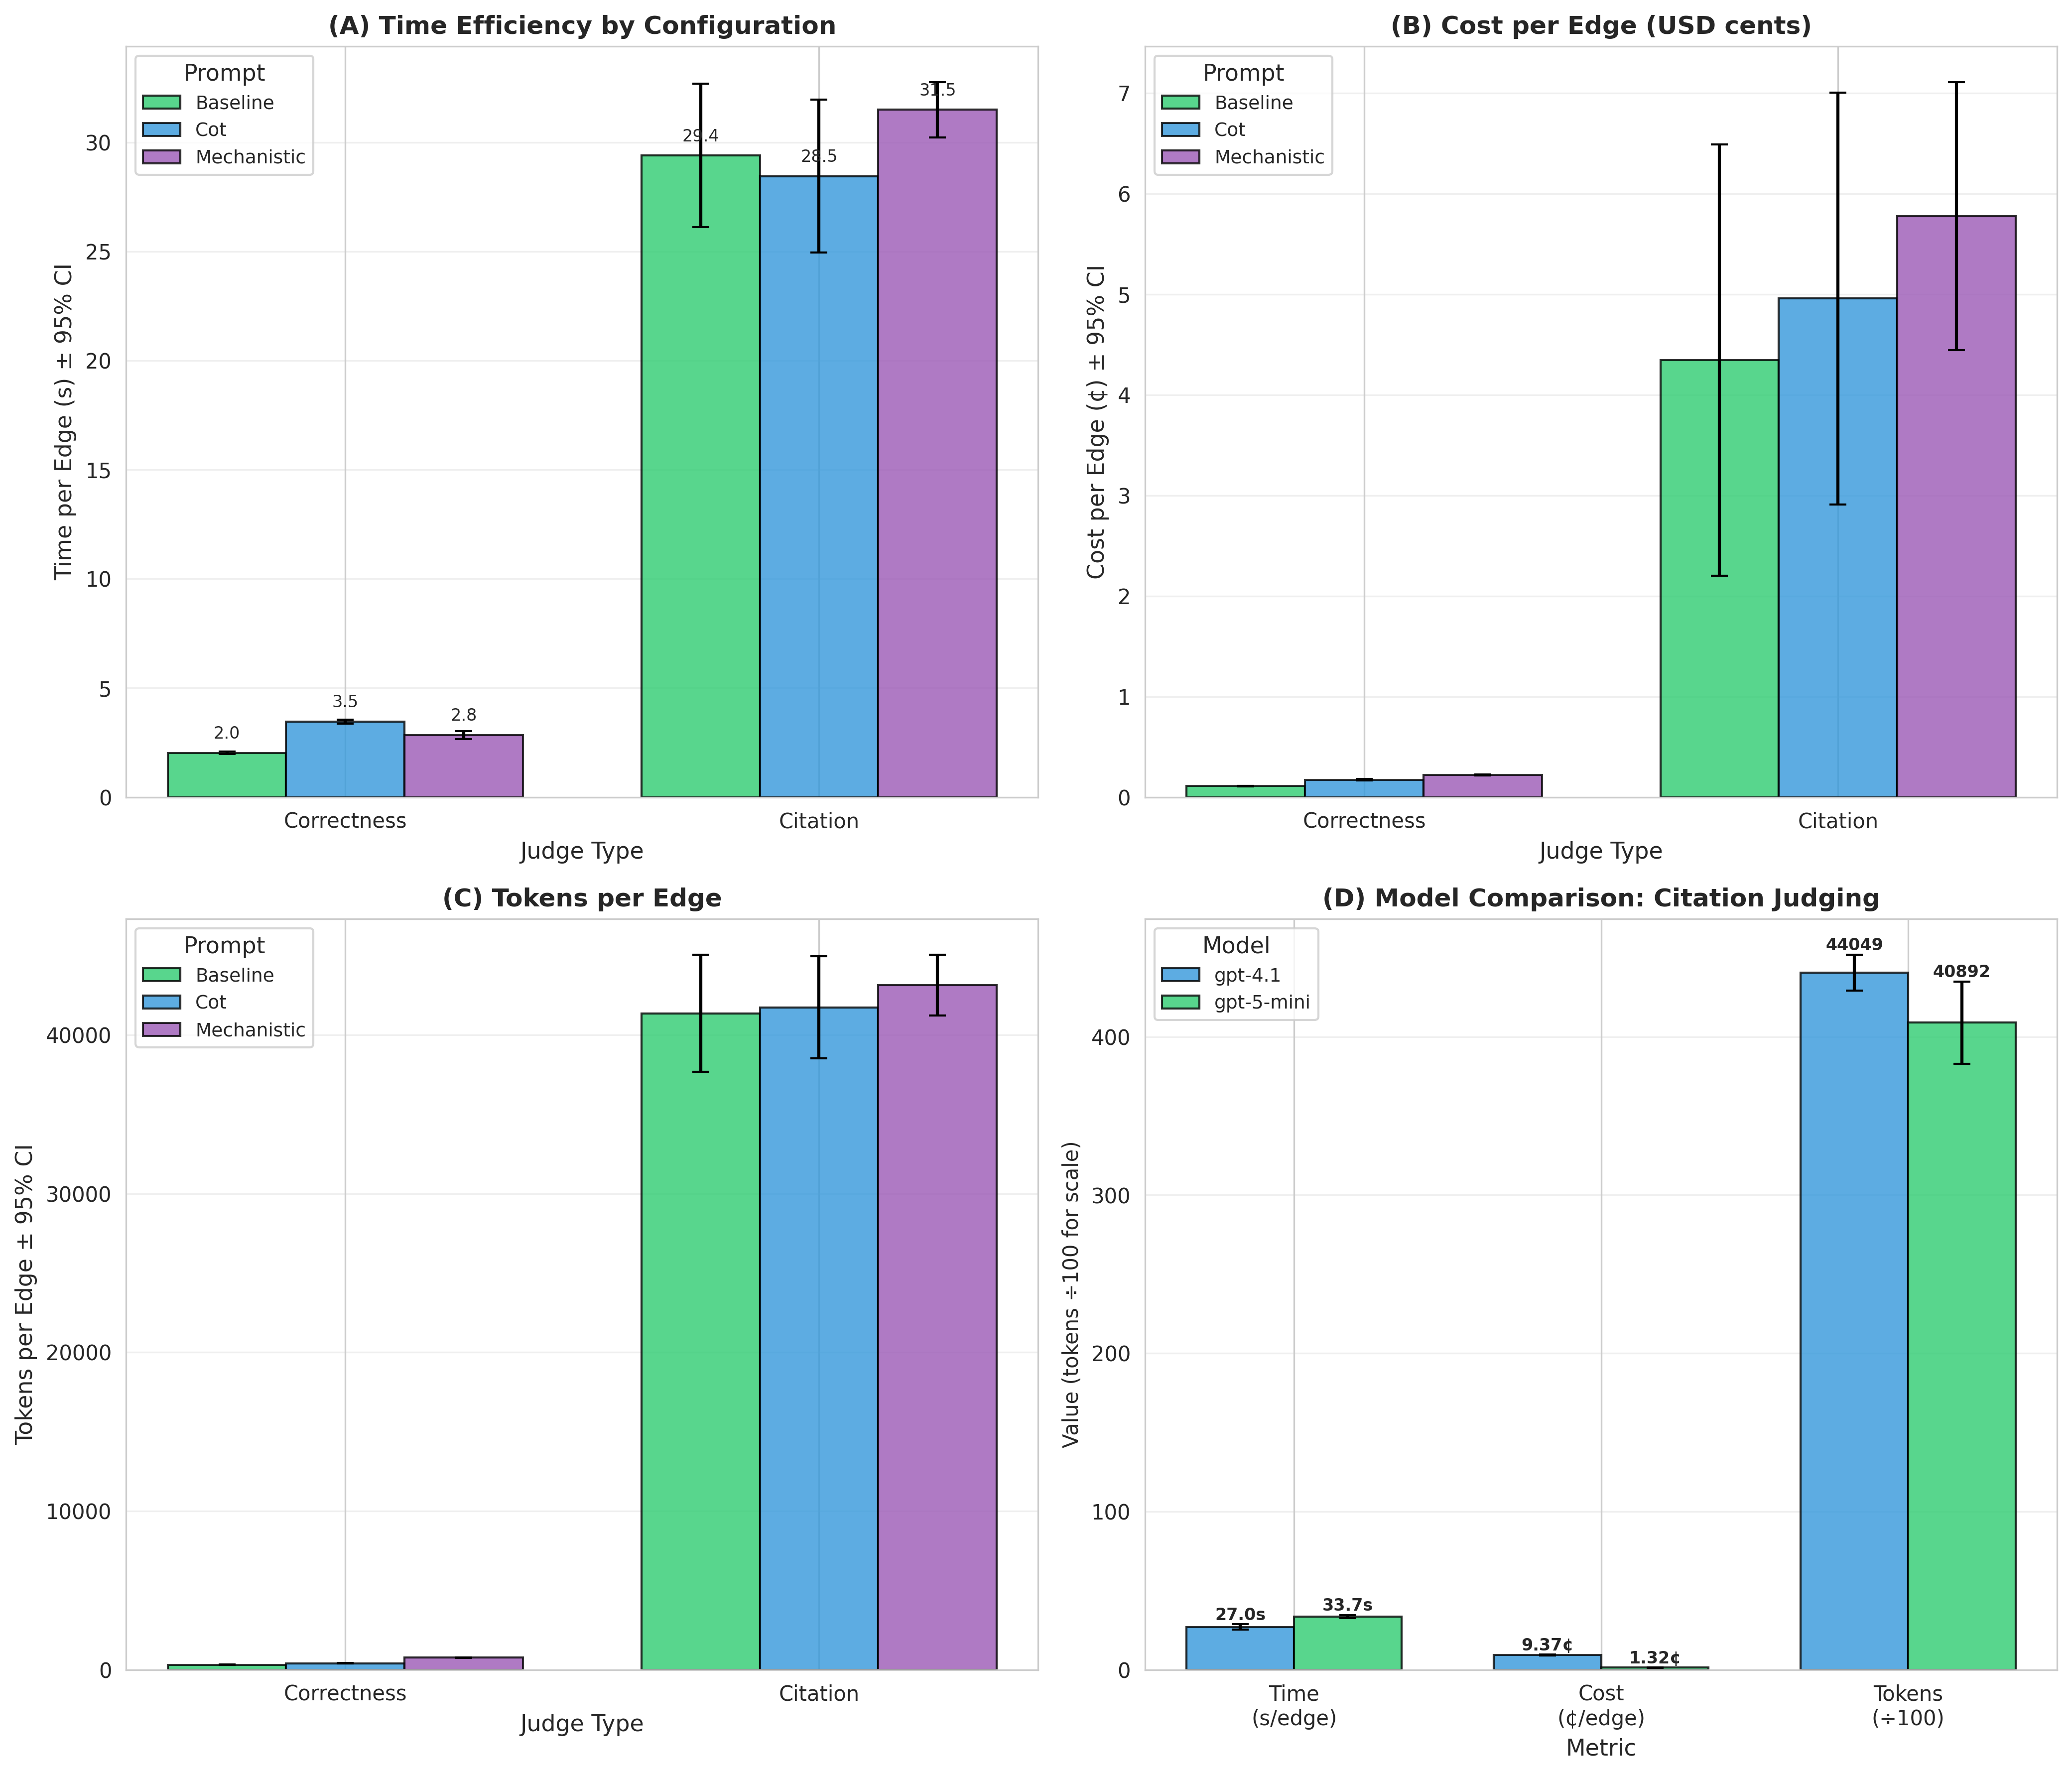
\includegraphics[width=1.0\textwidth]{../../final_runs/time_and_cost_scaling/figures/figure2_configuration_comparison.png}
\caption{Computational efficiency by configuration (mean $\pm$ 95\% CI). \textbf{(A)} Time per edge: Citation judging ($30.1 \pm 1.4$ s/edge) vs. correctness ($2.8 \pm 0.2$ s/edge). \textbf{(B)} Cost per edge: Citation ($5.6$¢/edge) vs. correctness ($0.17$¢/edge). \textbf{(C)} Token usage: Citation requires $\sim$11$\times$ more tokens due to retrieved document context. \textbf{(D)} Model comparison for citation judging: GPT-5-mini achieves comparable time/tokens at 97\% lower cost than GPT-4.1. All error bars show 95\% CI.}
\label{fig:config_comparison}
\end{figure}

\begin{figure}[H]
\centering
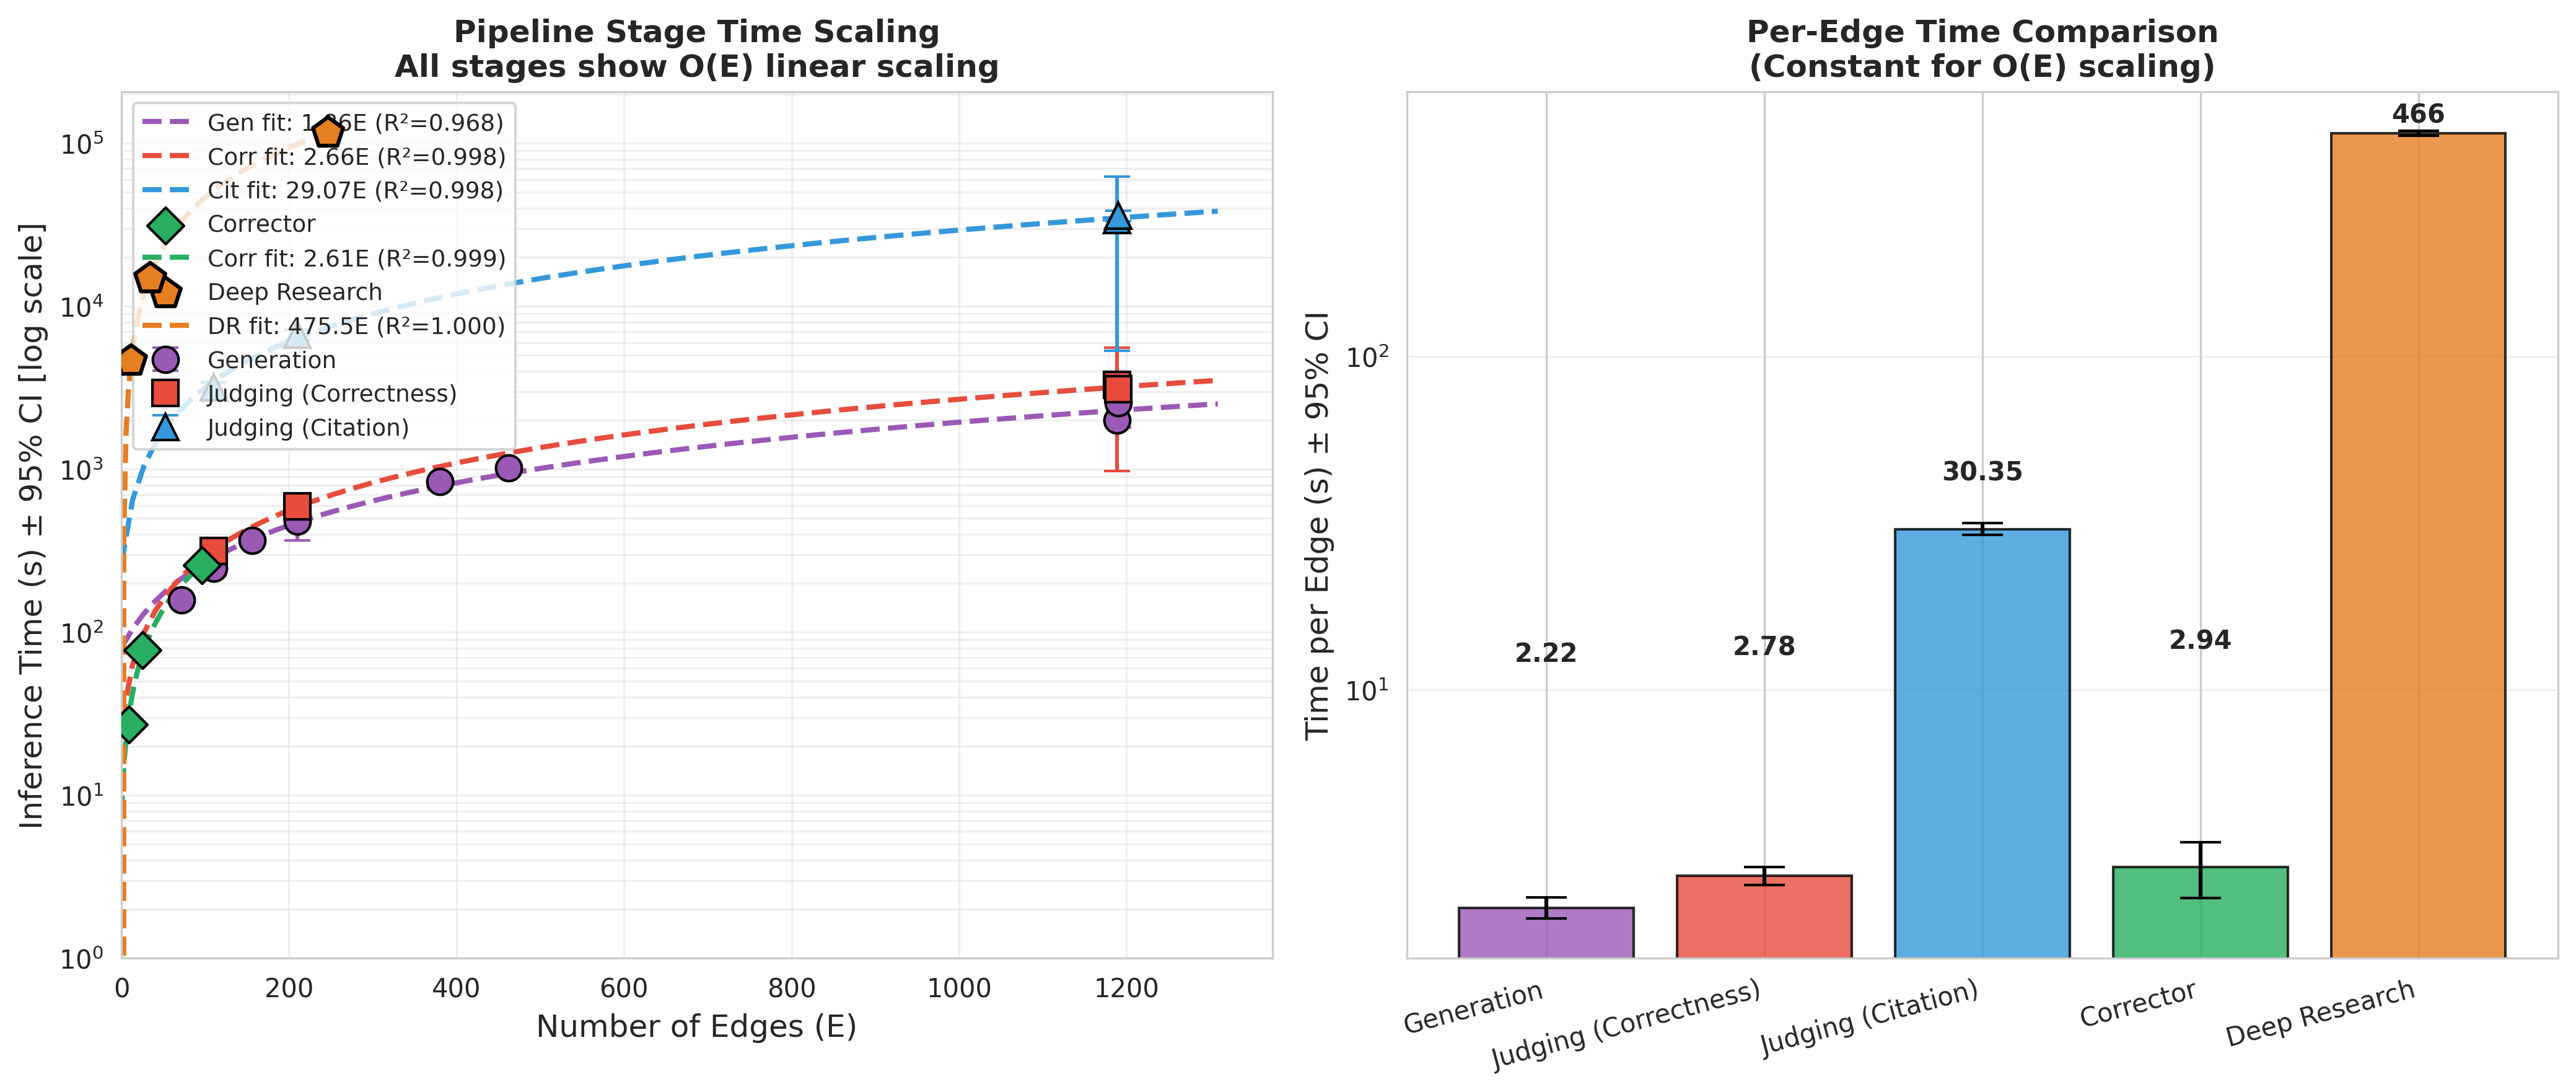
\includegraphics[width=1.0\textwidth]{../../final_runs/time_and_cost_scaling/figures/figure3_generation_vs_judging.png}
\caption{Wall-clock timing comparison across pipeline stages using GPT-4.1 for generation, judging, and correction. \textbf{Left:} Inference time vs.\ number of edges processed shows $O(E)$ linear scaling for all stages. Generation and judging process all edges in the CLD ($E = 110$--$1190$), while the corrector processes only candidate edges flagged for revision ($E = 9$--$96$, shown as green diamonds). \textbf{Right:} Per-edge time comparison shows generation ($2.2 \pm 0.5$ s/edge), correctness judging ($2.8 \pm 0.2$ s/edge), and correction ($2.8 \pm 0.4$ s/edge) have comparable costs, while citation judging ($30.1 \pm 1.4$ s/edge) dominates due to web search and document retrieval overhead. Error bars show 95\% CI.}
\label{fig:gen_vs_judge}
\end{figure}

\subsection{Token Cost Analysis}

\begin{table}[H]
\centering
\caption{Computational Efficiency Summary by Experiment}
\label{tab:scaling_summary}
\footnotesize
\begin{tabular}{llccccc}
\toprule
\textbf{Experiment} & \textbf{Model} & \textbf{Files} & \textbf{Edges} & \textbf{Tok/Edge} & \textbf{¢/Edge} & \textbf{Total (\$)} \\
\midrule
\multicolumn{7}{l}{\textit{RQ1a Judge Experiments (actual)}} \\
Corruption Citation & 5m & 28 & 13,800 & 43,313 & 0.73 & 100.14 \\
Ground Truth Citation & 4.1 & 43 & 20,143 & 46,053 & 9.65 & 1,944.70 \\
Corruption Correctness & 4.1 & 30 & 14,220 & 481 & 0.16 & 23.41 \\
Human Validation & 4.1 & 3 & 260 & 42,639 & 8.70 & 22.61 \\
\midrule
\multicolumn{7}{l}{\textit{RQ1b Corrector Experiments (estimated)}} \\
Synth Baseline & 4.1 & 14 & 5,275 & 993 & 0.33 & 17.41 \\
Synth CoT & 4.1 & 14 & 5,077 & 993 & 0.33 & 16.75 \\
Synth Mechanistic & 4.1 & 19 & 8,084 & 993 & 0.33 & 26.68 \\
GT Baseline & 4.1 & 18 & 9,058 & 993 & 0.33 & 29.89 \\
GT CoT & 4.1 & 9 & 5,609 & 993 & 0.33 & 18.51 \\
GT Mechanistic & 4.1 & 13 & 5,169 & 993 & 0.33 & 17.06 \\
\midrule
\multicolumn{7}{l}{\textit{RQ3 Deep Research (actual)}} \\
Deep Research & 5/5m & 3 & 285 & 246,893 & 86.67 & 247.00 \\
\midrule
\textbf{Total} & & & & & & \textbf{2,464.16} \\
\bottomrule
\end{tabular}
\begin{tablenotes}
\small
\item \textit{Note.} RQ1a costs from actual LLM Usage Stats. RQ1b estimated: correction + rejudging = 2$\times$ correctness tokens/edge ($\sim$497). RQ3 from actual Deep Research logs.
\item \textit{Pricing.} GPT-4.1: \$2.00/1M in, \$8.00/1M out. GPT-5-mini (5m): \$0.15/1M in, \$0.60/1M out. GPT-5: \$2.50/1M in, \$10.00/1M out.
\item \textbf{Key finding:} Deep Research dominates per-edge cost (247K tokens/edge, \$0.87/edge) due to multi-agent orchestration and iterative search.
\item \textit{Reproduction:} \texttt{python final\_runs/cost\_analysis/calculate\_all\_costs.py}, \texttt{compute\_dr\_costs.py}
\end{tablenotes}
\end{table}

\textbf{Practical Implications:}
\begin{itemize}[noitemsep]
    \item \textbf{Full pipeline cost:} For a 66-edge CLD (Emergency Dept), generation + correctness judging costs $\sim$\$0.29 and takes $\sim$6 minutes cumulative API time
    \item \textbf{Citation validation:} Adds significant overhead ($\sim$33 min cumulative, \$3.68 for GPT-4.1 or \$0.13 for GPT-5-mini)
    \item \textbf{Scaling:} Linear $O(E)$ scaling enables predictable cost estimation for arbitrary CLD sizes
\end{itemize}

\subsection{Parallelization Speedup}

To empirically verify parallelization benefits, we benchmark wall-clock time with varying worker counts on a standardized task: 34 correctness judging API calls (simulating the Depressive symptoms CLD edge count).

\textbf{Benchmark Configuration:}
\begin{itemize}[noitemsep]
    \item \textbf{Tasks:} Correctness judging (short prompts) and Citation judging (long prompts with retrieved citations)
    \item \textbf{Model:} GPT-4.1 (\texttt{temperature=0.3})
    \item \textbf{Simulated CLD:} Depressive symptoms (34 edges, 15 nodes)
    \item \textbf{Worker configurations:} 1 (sequential), 3, 5, 10 (parallel)
    \item \textbf{Runs per configuration:} 3 (for statistical robustness)
\end{itemize}

\begin{figure}[H]
\centering
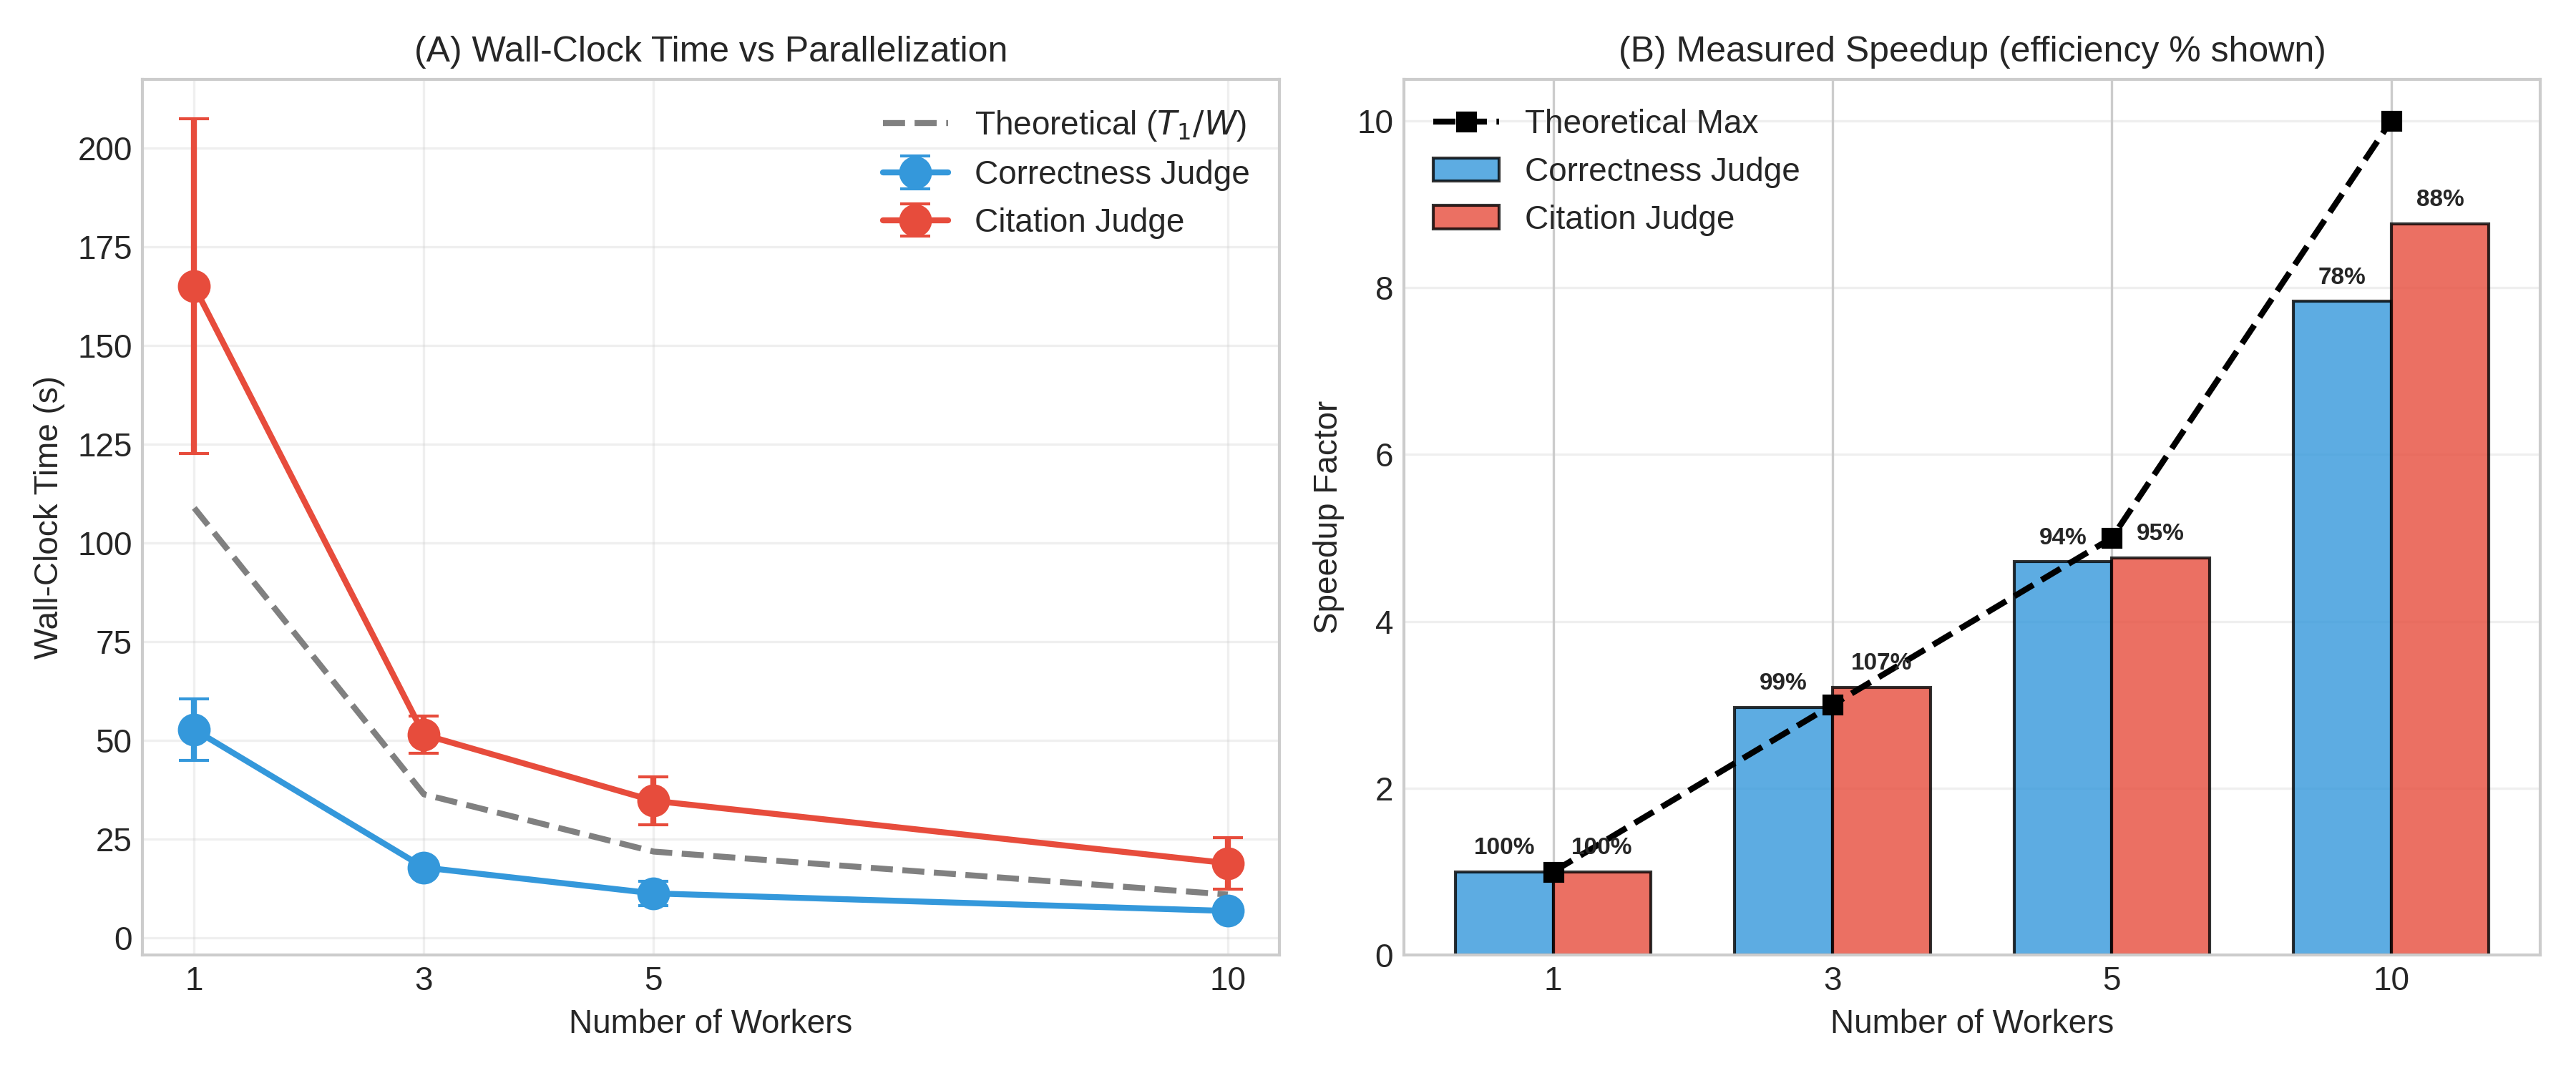
\includegraphics[width=1.0\textwidth]{../../final_runs/parallelization_benchmark/figures/parallelization_thesis_figure.png}
\caption{Parallelization benchmark comparing correctness and citation judging (34 edges, GPT-4.1, 3 runs per config, mean $\pm$ 95\% CI). \textbf{(A)} Wall-clock time: Citation judging (165s sequential) takes 3.1$\times$ longer than correctness (52.7s) due to longer prompts with retrieved citations. Both decrease with parallelization. Dashed line shows theoretical perfect scaling ($T_1/W$). \textbf{(B)} Measured speedup with efficiency percentages shown above bars. At 10 workers: correctness achieves 7.8$\times$ speedup (78\% efficiency), citation achieves 8.8$\times$ speedup (88\% efficiency). Citation judging shows slightly better parallel efficiency due to higher per-call latency dominating overhead.}
\label{fig:parallelization}
\end{figure}

\begin{table}[H]
\centering
\caption{Parallelization Benchmark: Wall-Clock Time and Speedup by Judge Type}
\label{tab:parallelization}
\begin{threeparttable}
\begin{tabular}{lcccccc}
\toprule
\textbf{Workers} & \multicolumn{3}{c}{\textbf{Correctness Judge}} & \multicolumn{3}{c}{\textbf{Citation Judge}} \\
\cmidrule(lr){2-4} \cmidrule(lr){5-7}
 & Time (s) & Speedup & Eff. & Time (s) & Speedup & Eff. \\
\midrule
1 & $52.7 \pm 7.8$ & 1.00$\times$ & 100\% & $165.0 \pm 42.4$ & 1.00$\times$ & 100\% \\
3 & $17.7 \pm 1.3$ & 2.97$\times$ & 99\% & $51.4 \pm 4.6$ & 3.21$\times$ & 107\% \\
5 & $11.2 \pm 3.1$ & 4.71$\times$ & 94\% & $34.6 \pm 6.1$ & 4.76$\times$ & 95\% \\
10 & $6.7 \pm 1.1$ & 7.84$\times$ & 78\% & $18.8 \pm 6.5$ & 8.77$\times$ & 88\% \\
\bottomrule
\end{tabular}
\begin{tablenotes}
\small
\item \textit{Note.} Model: GPT-4.1, temp=0.3. CLD: Depressive symptoms (34 edges). Time = wall-clock (mean $\pm$ 95\% CI, n=3). Speedup = $T_1/T_W$. Efficiency = Speedup/$W$ $\times$ 100\%.
\item \textbf{Key findings:} (1) Citation judging takes 3.1$\times$ longer than correctness due to longer prompts with retrieved citations (593 vs 174 tokens/edge). (2) Both achieve $\sim$8$\times$ speedup with 10 workers. (3) Citation has slightly better parallel efficiency (88\% vs 78\%) because higher per-call latency dominates overhead.
\end{tablenotes}
\end{threeparttable}
\end{table}
